
\documentclass[a4paper,11pt]{article}

\usepackage{amsmath,amssymb,amsfonts,amsthm}    % Typical maths resource packages
\usepackage{graphicx}                           % Packages to allow inclusion of graphics
\usepackage{hyperref}                           % For creating hyperlinks in cross references
\usepackage[authoryear]{natbib}                 % literature reference style
\usepackage{url}
\usepackage{alltt}
\usepackage{listings}
\usepackage{rotating}
\usepackage{cite}

\usepackage{multicol}

\usepackage{multirow}
\usepackage{graphicx}
\usepackage{subfig}
\usepackage{geometry}                % See geometry.pdf to learn the layout options. There are lots.
\geometry{a4paper}                   % ... or a4paper or a5paper or ... 
%\geometry{landscape}                % Activate for for rotated page geometry
\usepackage[parfill]{parskip}    % Activate to begin paragraphs with an empty line rather than an indent
\usepackage{graphicx}
\usepackage{subfig}
\usepackage{amssymb}
\usepackage{amsmath}
\usepackage{epstopdf}
\usepackage{multicol}
\usepackage{amsmath}
\usepackage{listings}
\usepackage{float}

\usepackage{multirow}
\usepackage{color}


% -------------------------------
\usepackage{natbib}% --- some layout definitions ---
% -------------------------------

% define topline
\usepackage[automark]{scrpage2}
\pagestyle{scrheadings}
\automark{section}
\clearscrheadings
\ohead{\headmark}
\cfoot{\pagemark}

% define citation style


% define page size, margin size
\setlength{\headheight}{1.1\baselineskip}
\voffset=-3cm
\hoffset=-3cm
\textheight24cm
\textwidth16.5cm
\topmargin1cm
\oddsidemargin3cm
\evensidemargin3cm

% define line line spacing = 1.5
\renewcommand{\baselinestretch}{1.5}

% define second level for `itemizing'
\renewcommand{\labelitemii}{-}

% --------------------------------------
% --------------------------------------
% --------------------------------------
% --- the structure the tex document ---
% ---  (this our recommendation) -------
% frontmatter:
%   - titlepage (mandatory),
%   - acknowledgement,
%   - abstract,
%   - table of contents (mandatory),
%   - list of abbreviations (not mandatory),
%   - list of figures (not mandatory),
%   - list of tables  (not mandatory) .
%
% body of the thesis (the structure of the thesis body is not mandatory, but the list of literature is mandatory):
%   - introduction,
%   - methods,
%   - data,
%   - results,
%   - conclusion,
%   - literature (mandatory),
%   - appendix (figures, tables).
%
% last page:
%   - declaration of authorship (mandatory).
% --------------------------------------
% --------------------------------------
% --------------------------------------

\begin{document}

% -------------------------------
% --- frontmatter: Title page ---
% -------------------------------
\thispagestyle{empty}

\begin{center}
\vspace*{\fill}

    {\Large{\bf Concept of an mobile assisting system for multi-sensor buildings-observation}} \vspace{0.5cm}
    
    {\Large{Entwurf eines mobiles Assistenzssystem für multisensorische Bauwerksüberwachung}} \vspace{0.5cm}


    {\normalsize EXPOSE: Master Thesis Euteneuer}\\\vspace{0.5cm}
    {\normalsize Technische Universität Berlin \\
    Institute für Geodäsie und Geoinformationstechnik\\
	Fachgebiet Methodik der Geoinformationstechnik\\
	superviesd by:\\	
	Prof. Frank Neitzel\\
	Thomas Becker}\vspace{1cm}

    {\normalsize by \\\vspace{0.5cm}
    {\bf Frieder H. Euteneuer}} \vspace{1cm}
		

    {\normalsize Berlin, \today}
\vfill
\end{center}




% ------------------------------------
% --- frontmatter: Acknowledgement ---
% ------------------------------------
\newpage
\pagenumbering{roman}   % define page number in roman style
\setcounter{page}{1}    % start page numbering
%\input{acknowledgement}

% -----------------------------
% --- frontmatter: Abstract ---
% -----------------------------
%\newpage
%\input{abstract}



% -----------------------------
% --- frontmatter: Contents ---
% -----------------------------
\newpage
\tableofcontents
%\clearpage


% ----------------------------------------------------
% --- frontmatter: List of Figures (not mandatory) ---
% ----------------------------------------------------
\newpage
\addcontentsline{toc}{section}{List of Figures}
\ohead[]{\rightmark}
\listoffigures


% ---------------------------------------------------
% --- frontmatter: List of Tables (not mandatory) ---
% ---------------------------------------------------
\newpage
\addcontentsline{toc}{section}{List of Tables}
%\listoftables



% -------------------------------
% --- main body of the thesis ---
% -------------------------------
\newpage
\setcounter{page}{1}    % start page numbering anew
\pagenumbering{arabic}  % page numbers in arabic style
\setcounter{secnumdepth}{4}


% 	PASTE HERE YOUR RESULT DOCUMENTS SEPARATED WITH NEWPAGES AS YOU CAN SEE BELOW
% 	AN ORDERING BY THE TWO PHASES AND BY THER THREE GROUPS WOULD BE USEFUL
%	--> PHASE 1; GROUP1; GROUP2; GROUP3; PHASE2; GROUP1 ...
%
%EXAMPLE
\part{Data Acquisition, Data Integration and Creation of LOD3 Model}
\newpage

\chapter{ %group 1
\section{Group 1 - Extraction of energy relevant attributes from 3D city model}
}
\subsection{Introduction}
The task for group 1 in phase 1 was to specify energy relevant attributes and try to calculate or extract them from the semantic city model.\\
First of all a connection to the database was necessary to establish, and the following three subtasks where reasonable to define.
With the specification of the energy relevant attributes inside of the database, a data basis for the different algorithms was created. This algorithms can be differentiated into data analysis algorithms basing on the pure values stored in the database and geometry analysis dealing with the geometry information in the database.\\
Our work was restricted to the area of Berlin Moabit, a small subset of the full Berlin model. For the Java algorithms the database information where exported as .gml files and the obtained output was saved as .csv files, which were able to be re-uploaded to the database. All data kept their necessary identifier.\\
As important values for an energy atlas following parameter where determined:
\begin{itemize}
\item Airvolume of building to be able to calculate the Surface-to-Volume-Ratio
\item Number of storeys which can be calculated by using the average storey-height of the specific building
\item Orientation of the wallsurfaces of each building to get information about neighbourhood relations between buildings and inner- and outer walls
\end{itemize}

\subsection{Data Analysis}
Each building stored in the database contains at least one groundsurface, one roofsurface and three wallsurfaces. Based on these information, the volume of the buildings, the orientation of the walls (whether it is a outer or neighbouring wall), therewith also the surface-to-volume-ratio and the outer-wall orientation for sunlight-heating-effects can be calculated. Also necessary for the average storey height and important for the calculations is the building’s function as it is residential, public or industry.\\
Moreover, we identified some missing energy relevant data like the building's year of construction. With this it is possible to estimate the building's material, the mean size of windows, the type of windows, and the mean story height. In addition, the topological relations between buildings are missing, as well as the number of people living in the building resp. number of flats, and the behaviour classes of the people living in the building (to estimate their energy consumption).

\subsection{Geometry Analysis}
In the geometry analysis we mainly focused on the surface area to volume ratio as well as the outer orientation of the walls. Carrion \citep{carrion2010} defines the surface area to volume ratio as follows:
\begin{quote}
"The S/V is the ratio of the aggregated area of all surfaces which transmit energy to the surrounding (wall surfaces touching other buildings are not considered) and the volume of the building."
\end{quote}
To calculate the S/V ratio, we created two subtasks. One task is to calculate for each building the area which is touching neighbouring buildings as well as to calculate the sum of all surface areas of one building. The second task is to calculate the volume of each building.

\subsection{Calculation of wall-surface intersection}
Important to know is, that the S/V does not include wall surfaces touching other buildings, and therewith those wallsurfaces must be detected using the information which are stored in the database. For this issue the following workflow to calculate wall surfaces which are not touching other buildings was developed:
\begin{enumerate}
\item Calculate neighbouring buildings
\item Calculate area touching other buildings (for each building)
\item Calculate sum of surface areas (ground-, roof-, wallsurfaces)
\item Subtract intersecting area with neighbouring building from sum of surface areas
\end{enumerate}

\subsubsection{Calculate neighbouring buildings}
The calculation of neighbouring buildings is done, to minimize the candidate set for the calculation of the intersection of two buildings. Two buildings are neighboured if the wall surfaces of the two buildings are within a certain distance, and the angle between wall surfaces is smaller than a defined threshold (see figure \ref{fig:neighbours3d}). 
Since we did the calculation in Java with the JTS Topology Suite (JTS), the problem was that JTS is not able to do calculations on 3D geometries. A workaround is to make the assumption, that the wall surfaces are vertical and parallel to each other. Then a projection of the walls into 2D can be done by ignoring the Z coordinates.
\begin{figure}[h]
	\centering
 	 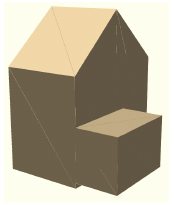
\includegraphics[scale=0.35]{phase1/group1/neighbours3d.png}
	\caption{Neighboured buildings in 3D.}
	 \label{fig:neighbours3d}
\end{figure}
This means, every wall surface becomes a linestring (see figure \ref{fig:neighbours2d}).
\begin{figure}[h]
	\centering
 	 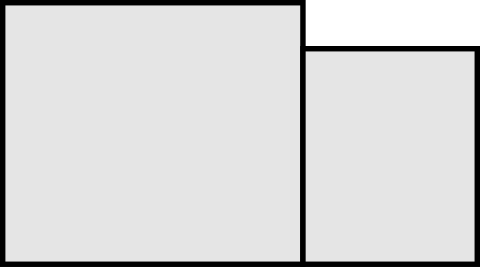
\includegraphics[scale=0.8]{phase1/group1/neighbours2d.png}
	\caption{Neighboured buildings in 2D.}
	\label{fig:neighbours2d}
\end{figure}
Then we can test if two walls represented by linestrings are within a certain distance and the angle between the linestrings is smaller than a threshold using JTS.

\subsubsection{Calculating area touching other buildings}
After determining if two buildings are neighboured, it is possible to calculate the intersection area of touching wall surfaces. Since JTS is not able to do calculations on 3D geometries, as mentioned above, the walls need to be transformed to 2D again. Therefore the coordinate system has to be transformed so that the wall surfaces are lying in the YZ-plane. Then, the X coordinate can be ignored and the intersection of the two walls can be calculated.\\
To rotate the coordinate system so that the wall surfaces are lying in the YZ-plane, the normal vector of one of the two walls has to be calculated. With this the rotation angle $\alpha$ can be calculated as the angle between the normal vector on the vector [1 0 0], which is the normal of the YZ-plane. Then both wall surfaces are rotated with this rotation angle $\alpha$. Figure \ref{fig:rotation_matrix} shows the used rotation matrix.
\begin{figure}[h]
	\centering
 	 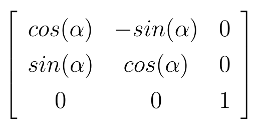
\includegraphics[scale=0.5]{phase1/group1/rotation_matrix.png}
	\caption{Rotation matrix used for calculating intersection.}
	\label{fig:rotation_matrix}
\end{figure}
If these rotated surfaces are intersecting, the real world surfaces are intersecting, too. Thus, the intersection of the rotated surfaces can be calculated as in the following listing:\\
\begin{lstlisting}[language=Java]
Geometry intersection=polygon.intersection(polygonNeighbour);
if (intersection instanceof com.vividsolutions.jts.geom.Polygon) {
  com.vividsolutions.jts.geom.Polygon intersectionPolygon 
  = (com.vividsolutions.jts.geom.Polygon) intersection;
  // unit is m^2
  intersectingArea = intersectionPolygon.getArea();
}
\end{lstlisting}

\subsubsection{Overall- and sharing wall area}
This is followed by the area calculation of the wall-, roof- and groundsurfaces for each building. These surface areas are summed up to get the overall surface area of each building.
These results (the surface areas of each building (building id)) are written to a .csv file to be able to import it back into the 3D city model database. Table \ref{table:result shared wall surfaces} shows some sample results.
\begin{table}[b]
\centering
\begin{tabular}{c  c  c}
building\_id & surface\_area & shared\_wall\_area\\
\hline						
BLDG\_0003000000432cd8 & 234.99638499102912 & 45.46462674214126\\
BLDG\_0003000000432c80 & 1265.0716547126067 & 529.4226535306225\\
BLDG\_0003000f000858d0 & 2201.2130139165056 & 975.798086083496\\
...\\
\end{tabular}
\caption{Subset of result .csv file containing shared wall surfaces.} 
\label{table:result shared wall surfaces}
\end{table}

\subsection{Geometry Analysis - Building Volume}
The building's volume can be calculated using several different approaches. The task is to have a volume which is a good approximation of the real existing air volume inside of the building, because it will be used afterwards for some energy-flow calculations. Necessary also for an operatively used approach is the automatisation of the algorithm and the potential for for its embedding into the other code.\\
The following approaches have been tested and checked whether they fulfil the requirements:
\begin{enumerate}
\item SQL algorithm/query
\item FME Software
\item ArcMap Software - 3D Analyst
\item ArcMap Software - Buildings to DEM
\end{enumerate}


\subsubsection{Volume calculation 1. approach: SQL}
Using SQL (Structured Query Language) as a possibility to directly access the database and analyse the stored information is the first upcoming option. For the calculation several Oracle spatial functions have been used to get the building area. Multiplying this with the building's height which is already stored in the database leads to a good estimation of the building's volume.\\
But the differences between the building's roof structure leads to wrong estimations of a large percentage of the building's volume, because only one height can be taken from the database which is the distance between the ground up to the highest roof point. The figure \ref{fig:build_h} is showing a good example of a possible wrong estimation: The different building parts are stored using only one building identifier, and therewith only the height of the highest part is stored inside of the database.
\begin{figure}[h]
	\centering
 	 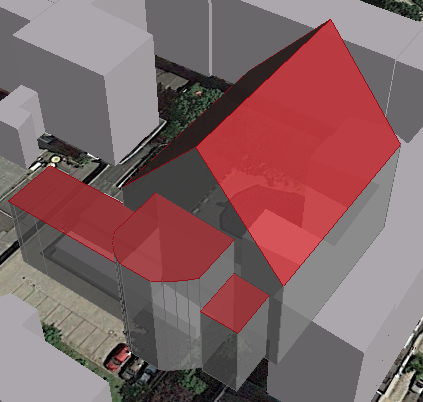
\includegraphics[scale=0.3]{phase1/group1/build_h.png} 
	\caption{Example of a more complex roof sturcture.}
	\label{fig:build_h}
\end{figure}

\subsubsection{Volume calculation 2. approach: FME}
The second approach was using the software FME (Feature Manipulating Engine). It’s FME Data Inspector shows the stored geometry and the buildings do not contain ground-, wall- and roofsurfaces (see figure \ref{fig:fme}). But the surfaces were represented as not connected so a building is not containing one closed geometry.\\
Since the FME workbench is very complex also a lot of errors occur, and therewith this approach is not really stable.
\begin{figure}[h]
	\centering
 	 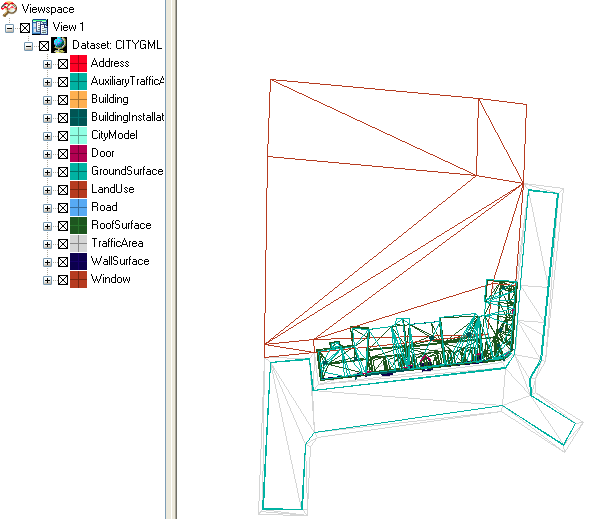
\includegraphics[scale=0.3]{phase1/group1/fme.png} 
	\caption{Visualisation of FME Data Inspector.}
	\label{fig:fme}
\end{figure}

\subsubsection{Volume calculation 3. approach: Arcmap}
The Software Arc Map offers an extension called 3D Analysed which can be used as an analysis tool for 3D objects.\\
In here it was possible to enclose the geometries of the buildings, but this procedure uses a shrinking of the building until every surface is completely touching its neighbours. Therewith the obtained volume of the building in systematically falsificated.

\subsubsection{Volume calculation 4. approach: Arcmap again}
For the last approach another functionality of Arc Map can be used: The creation of a rasterlayer for ground- and roof- geometries with the extension: "Add Buildings to DEM".\\
A complex sequence of operations have to be applied to first create a difference raster which is showing ground level and roof level and secondly calculating the volume using this raster.\\
For the automatisation the Arc Map Modelbuilder can be used. With this every step can be defined as an output and input of others. Figure \ref{fig:arcmap_raster} is showing the process.
\begin{figure}[h]
	\centering
 	 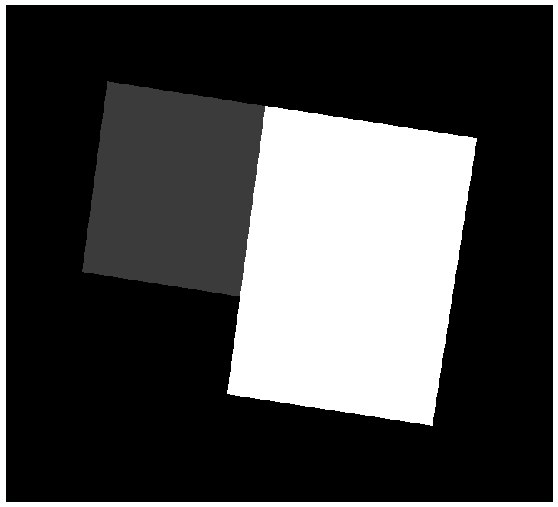
\includegraphics[scale=0.1]{phase1/group1/raster_ground.jpg} 
	 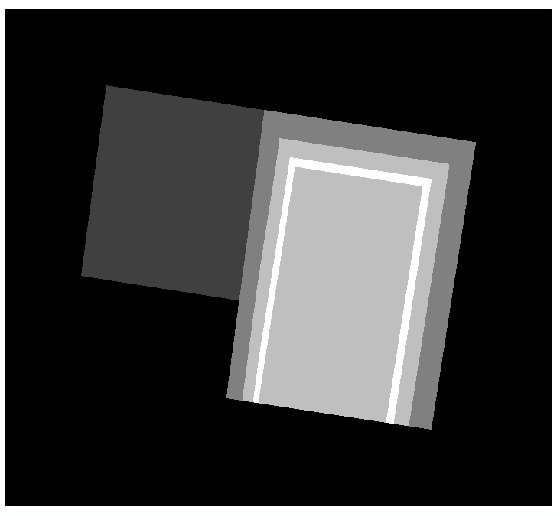
\includegraphics[scale=0.1]{phase1/group1/raster_roof.jpg}
	 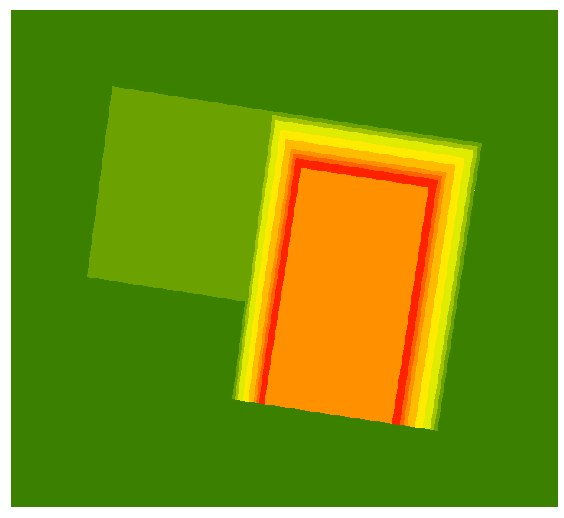
\includegraphics[scale=0.1]{phase1/group1/raster_diff.jpg} 
	 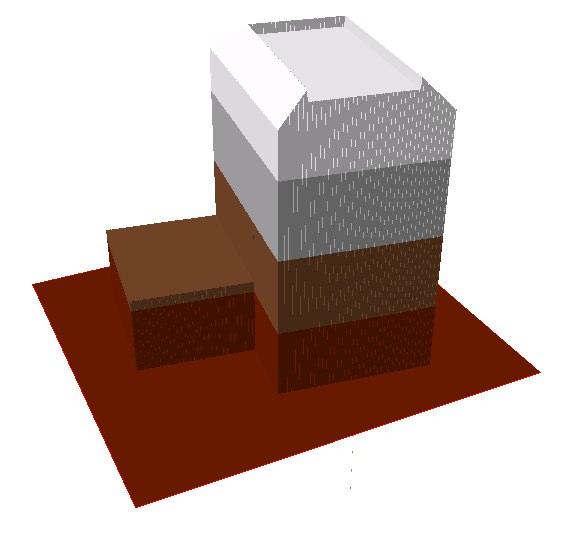
\includegraphics[scale=0.1]{phase1/group1/arcscene_tin.jpg} 
	 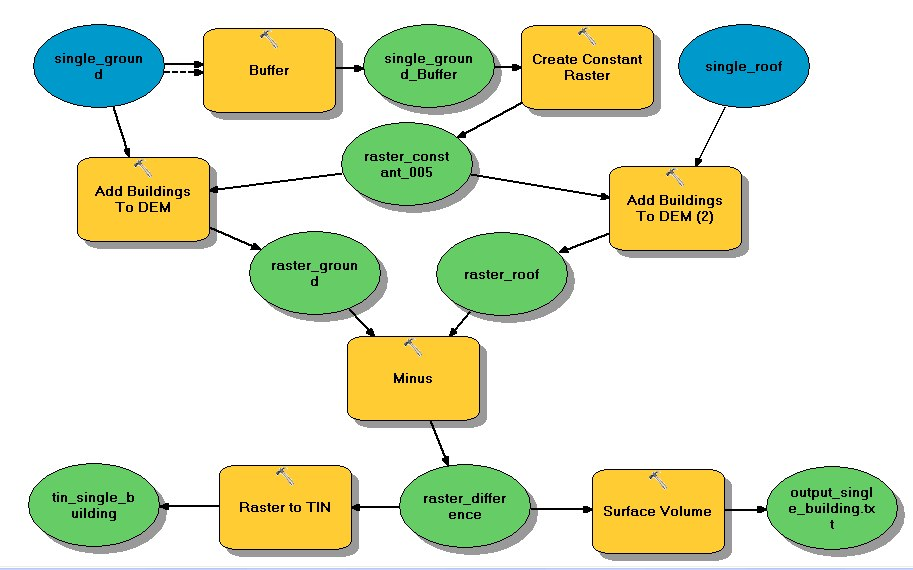
\includegraphics[scale=0.1]{phase1/group1/modelbuilder.jpg} 
	\caption{Visualisation of the 4th approach to calculate the volume.}
	\label{fig:arcmap_raster}
\end{figure}

\subsubsection{Volume calculation - Comparison}
Since our knowledge about the buildings is only depending on our data, a valid number of volume cannot be calculated without any statistical analysis of the buildings and the different calculations.\\
The table \ref{table:comparison_volume} shows a comparison of the different obtained results which.
\begin{table}[b]
\centering
\begin{tabular}{c  c  c}
Approach & calculated volume\\
\hline						
SQL & $10227m^3$\\
FME & no result\\
3D Analyst & $6000m^3$\\
Arc Map & $7400m^3$\\
\end{tabular}
\caption{Comparison of the different volume calculation procedures.} 
\label{table:comparison_volume}
\end{table}

\newpage
\chapter{
\section{Group 2 - Creation of 3D Model}}
\subsection{Introduction}
The modelation of Cities as 3D City model got more famous in the last years. Different appraoches from different domains to model the real world are common. The most famous domains, which deal with the creation of 3D models are Computer graphics, Architectural aided design and geoinformation science. In computer graphic and architecturel models only the geometry is represented. 3D models in geoinformation science store next to the geometry also semantics. This enables a user to use the 3D models for further investigations. This project deals with the enrichment of such a city model with an additional semantic layer, which contains energy related attributes. For this, the data of the 3D City DB of Berlin Moabit is used. Because the buildings are only available in LoD2, although LoD3 is required for a reliable energy demand estimation first LoD3 buildings are modeled. To create LoD 3 buildings different approach to model 3D building models with from building photographs are adopted. SketchUP is used for the 
modelation process. These models are enriched with the mentioned energy related attributes. Finally the new LoD 3 models are integrated in the 3D City DB.

\subsection{Workflow}
To model LoD 3 buildings and enrich them with energy realted attributes, the work can be splitted in three main parts, data acquisistion, 3D modeling and data integration. Figure \ref{fig:workflowph1} depicts the content of each project phase.

\begin{figure}[ht]
	\centering
	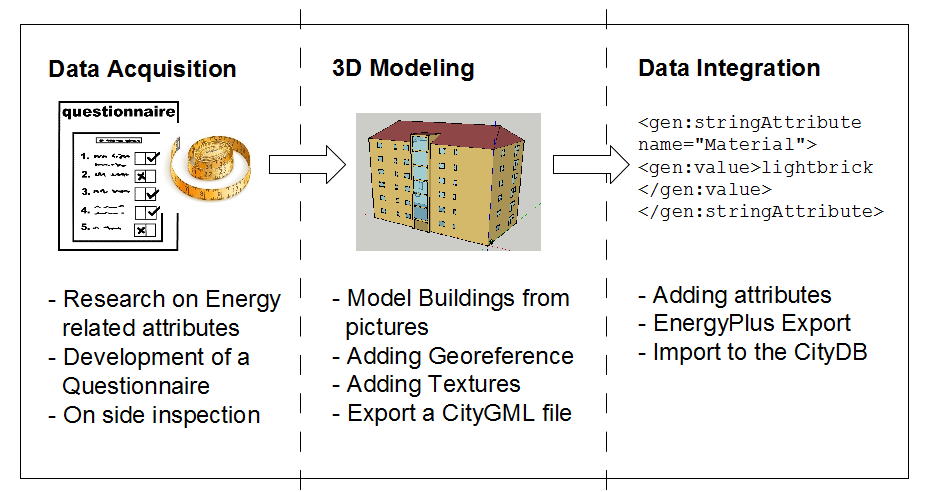
\includegraphics[width=0.8\textwidth]{phase1/group2/figures/workflow_phase1.png}
	\caption{Work packages for phase 1 of the GIS project}
	\label{fig:workflowph1}
\end{figure}

To model a LoD 3 building additional information about the geometry of e.g. windows, doors, as well as high resolution textures are necessary. For the integration of energy related attributes additional semantic data like the number of flats or the heating system have to be aquired. In order to collect this data a questionnaire was developed in the first step. \\
These questionnaire was used to acquire the necssary data for individual buildings by an onsite inspection. \\
The collected data is used to create LoD 3 models with SketchUP in phase 2. 
\\
Finally the models are enriched with the energy related attributes that are needed for the objective of this project.
Furthermore the new 3D models are exported as CityGML files and integrated into the 3D City Database. \\
In addition it was tried to export the building models as Energy Plus files, in order to run a Energy simulation with different input parameters. Because several problems with the SketchUp plugin Open Studio, which provides functions to generate Energy Plus consistent building models, were encountered it was not possible to export a Energy Plus file. \\
Therefore the report concentrates on the development of LoD 3 building models. 
\\
From the work packages the project schedule was created as guide to manage the project within a specific time frame. The project schedule can be found in annex1

\subsection{Data acquisistion}
\subsubsection{Development of a questionnaire}
The questionnare should cover all relevant questions to collect the data, which is needed for the creation of LoD 3 buildings models and the enrichment of these with energy related attributes. Therefore the requirments for LoD 3 building models have to be known. A LoD 3 building geometry comprises surface as well as windows, doors and balconies. Furthermore high resolution textures have to be available. To decide which energy related attributes are neccessary the "Kurzverfahren Energie Profil" of the Institut fuer Wohnen und Umwelt (IWU 2003) was used as reference. The questionnare can be seperated into eight parts:
\begin{itemize}
\item Address
\item General building attributes: Year of Construction, Number of flats, functionality, etc. (Figure \ref{fig:questionnaire}
\item Ground plan: sketch to get a better orientation
\item Adjacent buildings: neighboorhood sitiuation of the building (free standing, neighboor)
\item Basement
\item Roof: type, material, etc.
\item Window: Number of windows, U-values
\item Walls: Type, Insolation, Thickness, etc.
\item Doors: Material
\item Heating system
\item Additional notes
\end{itemize}

To simplify the field work for most questions predefined choices were created. For example seven roof types are proposed. The whole questionaire can be found in annex 2.

\begin{figure}[ht]
	\centering
	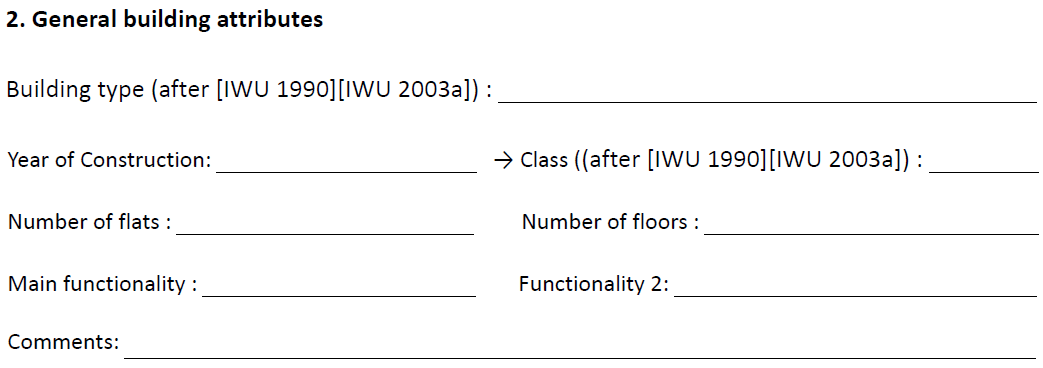
\includegraphics[width=0.8\textwidth]{phase1/group2/figures/questionnaire.png}
	\caption{Developed questionnaire}
	\label{fig:questionnaire}
\end{figure}


\subsubsection{Onsite inspection and data acquisistion}

The area of interest of the project is Berlin Moabit. In this area six buildings were selected based on different criteria like functionality, neighboring situation and year of construction. Therefore one free standing young office building, one old (1961) residential building with two adjacent buildings, as well as three residential buildings with one adjacent building were selected. \\
For this six buildings the questionnare was answered and several images were taken. Additionaly measuremnts were performed to determine the thickness of the walls and at least one reference height in order to scale the building models correctly. 
The images are later on used to model the buildings. Therefore images of each corner and each surface have to be taken as shown in figure \ref{fig:images}.

\begin{figure}[ht]
	\centering
	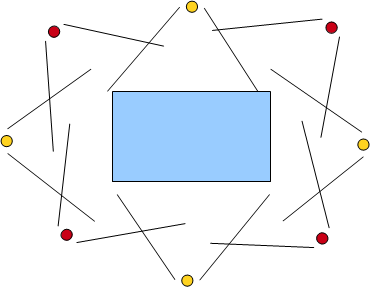
\includegraphics[width=0.5\textwidth]{phase1/group2/figures/images.png}
	\caption{Constrains on image acquisition}
	\label{fig:images}
\end{figure}

Because most of the buildings have adjacent buildings it was not always possible to take proper images of the building corners. Furthermore trees and cars were in the field of view.\\
The questionnaire is very detailed and covers all necessary data. In reality it has to be admitted that it was not possible to gather all information proposed by the questionnaire. For example it was only possible to collect information about the heating system for one building. The determination of year of construction of the buildings was not accuratly, too. The gathered information about the roof, e.g. type and material, the windows and doors, e.g. glazing, and walls is reliable.
\\
\\
The collected data is reorganized for furhter processings in a new Data sheet. It is attached as annex 3.

\subsection{3D Modeling}
The creation of LoD 3 building models is the major part of this project phase. To model the building SketchUp, a 3D modeling software, is used. In addition several SketchUP plugins such as Geores, a plugin to export the SketchUP models to CityGML, or OpenStudio, a plugin to generate Energy plus convienent models, are used. Furthermore FME is used to attach attributes to the CityGML models. The 3D City DB Importer and Exporter tool, which was developed by the geodesy and Geoinformation department of the Technical University of Berlin, is used to validate the created CityGML files and to integrate them in the 3D City DB.

\subsubsection{Creation of building model}
The 3D building modeling is based on the acquired images from different perspectives.To model consistent LoD3 buildings a work pattern was development, which was followed for all buildings. In the following the single steps are pointed out.
 
\begin{itemize}
\item Definition of left and right vanishing points.
\item Photos are calibrated based on the assumption that there are 90° angles.
\item Set the origin to a corner of the building. 
\item Set the scale. This is done by drawing a line representing the measured reference distance and scaling it to the real world length. Reference distances are measurments of the door, window or the 2D foot print which is extracted from the existing LoD 2 model in the 3D City DB.
\item Digitize the shape of the building from the current image as far as possible.Continue with the next images in the same way.
\item Windows and doors are digitized by creating openings in the. 
\end{itemize}

The roof of the building cannot be created from the acquired images. The shapes of the roofs are estimated from the satellite images of google earth and modeleld without reference.

\begin{figure}[ht]
	\centering
	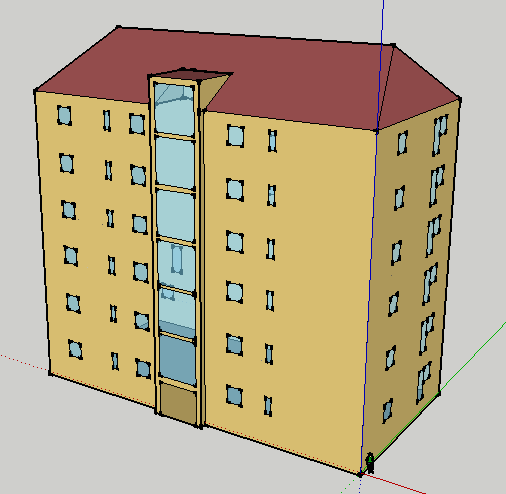
\includegraphics[width=0.5\textwidth]{phase1/group2/figures/Building_wiclef.png}
	\caption{Work packages for phase 1 of the GIS project}
	\label{fig:Building_wiclef}
\end{figure}

After the creation of the 3D model of a building the used images are projected on the surface of the models and used as textures. Because some images are highly distorted the textures don't correspond perfectly to the geometry. The following steps were followed to project the texture on the model.

\begin{itemize}
\item choose a picture
\item Mark the surface to which the texture should be applied 
\item Press the buttion "project texture from photos" from the "Match-Photo"-Dialog
\end{itemize}

Four of the six buildings were modeled with this workflow.


\subsubsection{Handling Layers in SketchUP}

For a successful export to cityGML the features of a building have to organized in a sophisticated layer structure.
Different layers are created for the model in order to identify each surface and opening as a unique entity in the exported cityGML file. The layer is created with sketch up following some standard rules to make each layer unique with an id. The workflow used for creating the layers is as follows:


\begin{itemize}
\item Highlighted a particular surface or part of the building model 
\item Click on ``create layer'' from the window button in sketch up
\item Assign a layer name according to following rules
\end{itemize}

This is repeated for all the surfaces and all the building part of the model. Features of each surface could be grouped or ungrouped for a single surface. For the purpose of this project the building features are mostly grouped. 

To make the model compatible to the GEORES plugin of sketch up, the layer need to named according to some rules which will be explained in the following chapter.
All layers belonging to one building need to start with the same prefix, followed by a dot.
\begin{lstlisting}
building1.
\end{lstlisting}

For each wall, ground or roof surface an extra layer has to be created as subitems of the building and the given ids of the surfaces have to unique within the model.
\begin{lstlisting}
building1.wall1
building1.roof1
building1.ground1
\end{lstlisting}
 Surfaces belonging to one type can also be assigned to one layer, but they need to be grouped instead of the id,  a "s" indicates that there are grouped surfaces in the layer.  If a surface has subsurfaces (openings) like windows or doors it cannot be grouped and needs to be in an extra layer as shown above.
 \begin{lstlisting}
  building1.walls
building1.roofs
building1.grounds
 \end{lstlisting}

Openings must be either a door or windows and the layer name follows the same schema.
A unique id for each opening, or openings belonging to one surface can be grouped and assigned to one layer ending on "s".

\begin{lstlisting}
 building1.wall1.window1
building1.wall1.window2
building1.wall1.door1
building1.wall2.windows
building1.wall2.doors
\end{lstlisting}

\subsubsection{Geocoding and export to cityGML}

Geo location is the alignment of the building data to a known reference system, in order to represent the model in the true location in real space.  Georeferencing is very important in modeling and using the right reference coordinate system is very important so that the integration of the model can be done in the city model for compatibility and consistence reason. For the georeference of the building model the following steps have to be followed.
First of all the building has to be rotated. Therefore the directional angle of on side of the corresponding LOD2 is taken, to be able to rotate the new LOD 3 model in the right way. The position of the building is added during the export to cityGML using the GEORES Plugin for Sketch Up. Within the dialog box of the export the shift in east and north direction has to be filled in.

\subsubsection{Adding of generic attributes to the building} 

This is the phase where attributes are added to the model, using the FME software application. Different kinds of attributes are added to each building model, the generic attributes, the standard attributes, wall attributes and so on.  Different kinds of properties or instances are added to the building model as attributes. These properties vary from general information like building age, number of stories, energy related properties like u values and the wall to window ratio.

The U values for each building part are obtained from the Energieprofil Kurzverfahren (annex 3) which categorize the materials used. The U-value for the materials are based on the building age class. The u value is also known as the thermal transmittance which is the energy (W) transmitted through one $m^2$ of a material with a certain temperature difference between both sides. The unit of this value is [W/ (m²K)].
The window to wall ratio is computed and added as an attributes also. In the Energieprofil Kurzverfahren there is a reference for building classes and the window to wall ratio.

As mentioned above the software FME has been used to add the attributes to the building. To do so, following workflow has been developed by the group of students.

\begin{itemize}
\item creation of a writer
\subitem used format: City GML
\subitem dataset: the exported Citygml file
\subitem Workflow Options: Static Schema
\item Create a new Reader
\subitem select City gml as file
\subitem select your exported City GML file
\subitem select individual feature types
\subitem click ok
\subitem check all boxes
\subitem check also add to writer
\subitem click ok
\item Delete the writer you created first
\item Open the Feature Type Properties of the writer of a Surface you like (e.g. Wall Surface)
\subitem go to User Attributes
\subitem add a new name and chose citygml string as format
\subitem click ok
\item Double click the red arrow in front of the new added attribute
\subitem type in the value of the attribute
\subitem Set coordinate system
\subitem expand writer in navigator
\item set coordinate system to "DHDN.Berlin/Cassini"
\subitem expand "Parameters"
\subitem set "GML srsName" to "3068"
\subitem set "GML SRS Axis Order" to "1,2,3"
\item Click run
\end{itemize}

Following attributes have been created using this approach.
\begin{itemize}
\item Building
\subitem volume
\subitem height
\subitem no\_of\_floors
\subitem no\_of\_flats
\subitem total\_wall\_area
\subitem adjacentWall\_wall\_area
\subitem no\_adjacentWall\_wall\_area
\subitem roof\_area
\subitem window\_area 
\subitem heating\_system
\subitem no\_of\_inhabitants
\subitem basement (boolean)
\subitem ratio\_windowArea\_totalWallArea
\subitem ratio\_windowArea\_totalAreaWallWithWindows
\subitem ratio\_windowArea\_noAdjacentWallArea 
\subitem ratio\_windowArea\_floorSpace (floorspace = ground\_area * storeys)
\subitem citygml\_class
\subitem citygml\_function
\subitem citygml\_usage
\subitem citygml\_year\_of\_construction
\subitem citygml\_storeys\_above\_ground
\subitem citygml\_storeys\_above\_ground
\item Wall Surfaces
\subitem u value
\subitem material
\subitem thickness
\item Roof Surfaces 
\subitem u\_value
\subitem materials
\item Windows
\subitem u\_value
\end{itemize}



\subsubsection{Validation of City GML file and integration into the 3D city database}

The validation and integration was done by using the Importer-Exporter Tool developed by our institute. After setting up the connection to the 3d- city database the City GML file with the new Building has to be selected under the tab Import. Every setting is left on default setting. The validate button is clicked and the validation is done automatically starts the validation of the input file against the xml schema definition of the City GML application schema. After the validation the file is suitable for the import.  The button import is then pressed to integrate the model in the database.

\subsubsection{Visualization and presentation of model }

The visualization is done using goggle earth, the four different building are viewed in there different location in space. 
The results of the building model were presented below with all the major details of the models in sketch up after additional of all the attributes and projection of textures. Figure \ref{fig:kaiserin} shows one of the four building which have been modeled.
\begin{figure}[ht]
	\centering
	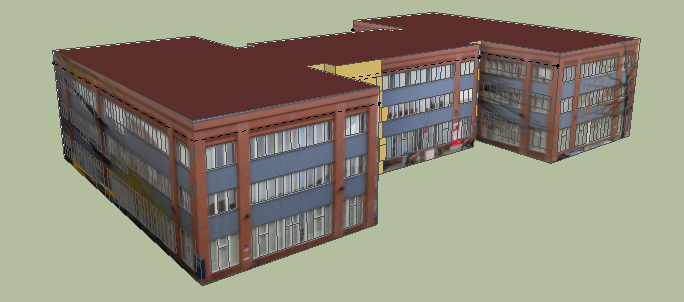
\includegraphics[width=0.8\textwidth]{phase1/group2/figures/kaiserin.png}
	\caption{Model of building located at Kaiserin-Augusta-Alle 10B}
	\label{fig:kaiserin}
\end{figure}


\subsection{Conclusion}
From the visualization of the results of the building model, it can be seen that the building model created had been used to replace the LoD 2 model, with this change the city gml model of berlin has been updated for four selected buildings to LoD 3 with useful energy attributes and generic attributes that can allowed for different query and simulations. The approach has seen compared to previous approach can be said to be cost effective and possible for implementation on small data set. This approach will not be suitable on large set of data because it might be very complicated and time consuming. It will be ideal to use this project approach for regular or periodic update of selected data or addition of new data of newly constructed building into the 3D cadastral. 






\chapter{
\section{Group 3 - Further Sources for Additional Data and Integration on 3D Models}
}%group 3

\subsection{Introduction}
The goal of this report is to describe the procedure performed by the group 3 for the phase 1 and 2 of the GIS-Project in the Winter Semester 2012/13.
The main task for phase 1 regards the search for further data and its integration on the data-model using an automatic or semi-automatic process. The operations involved a large number of data exchanging through different formats and a large number of  applications, such as SQL, ArcGis, FME and Excel were applied. Though, it is hard to establish an unique and solid procedure which could be systematically repeated.
After the integration of the required data, the indicators Apartments/Volume (m3) and Number of Residents/Apartment were calculated and, in the case of the first indicator, different values were obtained since they were grouped by the attribute Age of the Building.
The phase 2 comprises the actual estimation of the residential annual electricity consumption on the area of interest. Therefore, all integrated data from phase 1 is gathered in an appropriate algorithm, which relates households and annual electricity consumption.
The final result for the households average is 1.584, in contrast to the statistical one: 1.65 (Amt für Statistik Berlin-Brandenburg, 2011). That led for an average annual electricity consumption range of 2671 - 2931 kWh per apartment.
A further research towards a complete automation of the process is recommended and normally requires programmed scripts (e.g in Java) which might deal direct with both the stored data and the data to be integrated from other sources (e.g WMS and WFS), and also perform the final algorithm.
\subsection{Data Sources}
There are many sources of data available which can be integrated either directly by a simple spatial relationship or by joining operations which might become complex depending on the structure differences.\\ 
In the case of Berlin, the FIS-Broker database (http://fbinter.stadt-berlin.de) presents a large and spatially located amount of statiscal and survey data regarding social, economical and infra-structural fields. It is the most important source used during the accomplishment of the tasks.
The figure 1 elucidates the whole process divided into three steps – searching, processing and integrating:\\
\begin{figure}[ht]
	\centering
	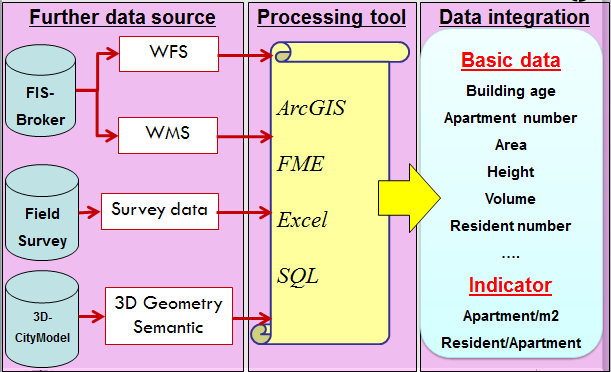
\includegraphics[width=0.9\textwidth]{phase1/group3/fig1.png}
	\caption{Data Workflow}
	\label{fig:figure1}
\end{figure}
As figure \ref{fig:figure1} shows, the sources of data consist basically on the FIS-Broker, the 3D City-Model, which provides all geometric and semantic required information, and the so called "Field Survey", consisting of a survey previously realized in the Moabit area that gathered information for random buildings regarding its number of apartments. \\
Depending on the application, many other sources can be integrated, enabling such a variety of possible calculations. The exact type of data depends also on the method to be used. The more detailed the algorithm, the more data is required. 
\subsection{Data Acquisition }
\subsubsection{WMS}

The WMS provides the web map services as a raster map. Normally, only the color information and legend are provided, but not the exact data. However, it is still an important data source and there are plenty of map services provided by WMS. In FIS-Broker database, most of data such as the building age group, proportion of different age group can be accessed by using WMS. 
In this project, a whole process of getting WMS data in FIS-Broker was created: \\
1. Get the link to URLfor WMS service from:\\
www.stadtentwicklung.berlin.de\\
2. Using ArcGIS connect to the WMS.\\
3. Set the coordinates system\\
4. Export map by choosing .tiff format in high resolution (300 dpi) and geotiff Tags\\
5. Combine the export map (Spatial Analyst Tools->Local->Combine)\\
6. Re-color raster data and make new legend\\
7. Zonal statistics as table\\
8. Join statistics table and new legend to the feature layer\\

The WMS information is saved in the feature layer after all these steps above. But maybe there are some errors in the boundary due to the data resolution. \\
\begin{figure}[ht]
	\centering
	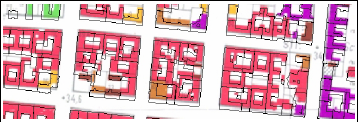
\includegraphics[width=0.9\textwidth]{phase1/group3/fig2.png}
	\caption{Mismatch of Overlap (Carrion, 2010)}
	\label{fig:figure2}
\end{figure}
\subsubsection{WFS}

The WFS  is the short term for Web Feature Service in which the graphical features can be requested from the services. Both geometry and semantic data are provided by WFS. Therefore, not the color information, but the database can be easily requested by the users compare to WMS. For example, in WMS, the information of building age is given in a time period which is shown in the legend, while in WFS it is provided the exact construction year, as a vector data, which is more specific and useful. \\
To get WFS data, several steps are needed  as follows:\\

1. Applying FME Intergration Console - add FME extension to ArcGIS

2. Add FME connection

3. Select WFS data Format

4. Set parameter.\\

Some feature data like building and statistical block as well as semantic data like number of residents in each block are extracted from WFS. However, the WFS services are not commonly open. The FIS-Broker WFS services is not availabe anymore available, due to security reasons.

\subsubsection{Field Survey}
The energy consumption have a tightly relationship with number of apartments. Therefore a field survey for apartment number is necessary. This survey is done based on different building age group. For each building group, at least 10 buildings were selected to count the number of apartment by counting the ring bells.
\subsubsection{CityGML}
Also some useful data can be obtain from CityGML, especially 3D geometry data, such as the footprint area and building height. Because only the residential volume is important in this project, the height of the building is calculate by removing the roof height.
\subsection{Integration}
The aim of Phase I is to get two important indicators: Apartment/Volume(m3) and Resident/Apartment. To calculate these two indicators, not only the data from different data sources is required, but also different tools (FME, ArcGIS, SQL, Excel) should be integrated together.
\subsubsection{Age of Buildings}

The attribute age of buildings specifies the exact year of construction for the buildings. For cities like Berlin which have a long history, the building age may vary from more than 100 years to recent 1 or 2 years. As architectural properties might not vary so deeply during years or even decades, this attribute is better represented by a range of values. \\

Therefore, the attribute age class was separated into 6 groups: 1889-1918, 1919-1945, 1946-1961, 1962-1974, 1975-1993 and 1994-2012.\\
\subsubsection{Apartment Number / Volume}
The number of apartment is the key value for the next steps. As it is impossible to do the survey for all buildings in the test area, this indicator was introduced. It is calculated from the field survey data and then can be easily gotten the apartment number of other buildings by multiplying this indicator with the building volume.

As a further data to be attached on the calculations, a survey was performed on the area of interest, with the goal of obtaining the number of apartments on the region. Thus, the survey data provides the counting of the ring bells for a selected group of buildings.

The process to join all the information must contain an export of the surveying data on the database. Then, the GMLID have to be joined accordingly – this is realized by the address of the buildings, as both the surveying data and the data model provide it. 

The following script is an example of a join by the address. It shows basically the final step, once the surveying data is already imported on the data model:
\begin{lstlisting}
select  street, house_number, apartment, a.id,
b.building_id,co.gmlid
from join_surveying js
inner join address a
on js.strasse=a.street and js.hnr=a.house_number join
address_to_building b
on a.id=b.address_id join cityobject co
on b.building_id=co.id;
\end{lstlisting}

As the footprints are  to provide the area of the buildings, one must aggregate the height information. A close look on the database highlights the existence of three different heights per building:
\begin{itemize}
\item Measured\_Height (Hm): representing the total height of the building
\item H\_Trauf (Ht): the lower height of the roof
\item H\_First (Hf): the upper height of the roof
\end{itemize}

So, the real height (Hr) is calculated through the following relationship:
\begin{align}
Hr=Hm-(Hf-Ht)
\end{align}


The real volume for each building is trivially obtained from the multiplication of the footprint area with the real height. Then, the indicator " apartment Number / Volume(m3)” is performed like:\\
\begin{align}
I = \frac {\sum\limits_{k=1}^n T_{k}}{\sum\limits_{k=1}^n V_{k}}
\end{align}


Where:\\
I = Indicator (Apartment number / Volume(m3))\\
T = number of apartments of building k\\
V= volume of building k\\
n = total surveyed buildings\\
\\
Afterwards, the above procedure is expanded. Each building age class receives a different indicator, as they present different periods of construction and, therefore, different architectural configurations which renders different results.\\

It is important to mention that the indicators inherit an expectation "behave". It is well known that older buildings used to have less apartment for the same amount of volume. Another socio-economic issue is related to the period right after the second World War. As the demand for new buildings was very high due to the destruction caused by the war, the short period after 1945 should present the highest indicators. \\

Also, the integration of the surveying data presents some mismatches from real data to the 3D Model. Some buildings have more than one address and vice-versa. Some garages are integrated on the buildings and, therefore, would be part of the volume calculation.\\

In order to avoid mismatches and to build reliable indicators, some unclear data were not taken into account. For the next survey missions, it is recommended to take a brief look on the 3D Data Model before going to the field, so that only reliable buildings could be selected.



\subsubsection{Number of Inhabitants}

A very important data for input in energy simulations is the number of inhabitants of the residential area of interest. Once the city model supports semantic information about the usage of the buildings, it is possible to split the inhabitants inside the buildings, and so, have an estimation of the households.\\
For this task, a WFS was provided containing the total amount of inhabitants per block. In order to obtain the total amount of inhabitants per building, a weighting by an approximation of the building volume was performed.

\begin{figure}[ht]
	\centering
	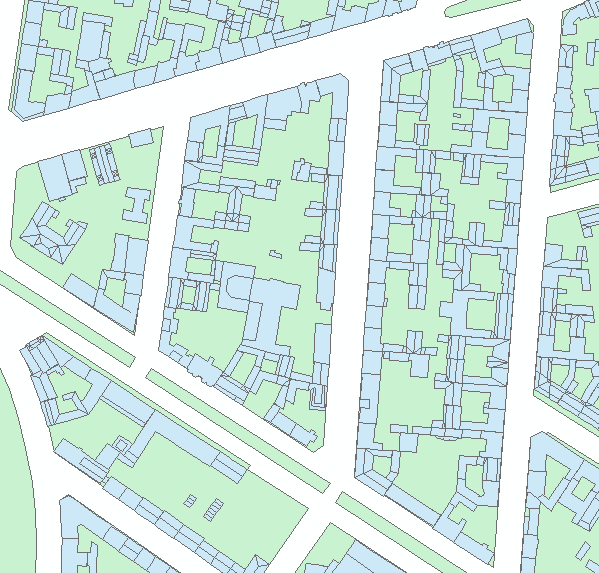
\includegraphics[width=0.8\textwidth]{phase1/group3/fig3.PNG}
	\caption{Building Footprints X Block (Self Made)}
	\label{fig:figure3}
\end{figure}

In order to calculate the number of inhabitants or residents per building, a previous selection is performed on the database, returning only the buildings which present residential purpose. As the buildings are semantically defined also by its function of usage, based on OSKA(Objektschlüsselkatalog – 2003) the following script was performed: \\

\begin{lstlisting}
select  b.id,co.gmlid, b.function, b.measured_height,
a.street, a.house_number
from cityobject co , building b, address a, 
address_to_building ab
where b.id=co.id and b.id=ab.building_id and 
ab.address_id = a.id and (
b.function='1373' or b.function='1331' or b.function='1311'
or b.function='1372' or b.function='1399' or b.function='1379'
or b.function='1381' or b.function='2199' or b.function='1301'
or b.function='1361' or b.function='1341' or b.function='1221' 
or b.function='1321' or b.function='1374' or b.function='1371'
or b.function='1231' or b.function='2131'  
or b.function='2121' or b.function='2101'   
or    b.function='2141');
\end{lstlisting}

\begin{figure}[ht]
	\centering
	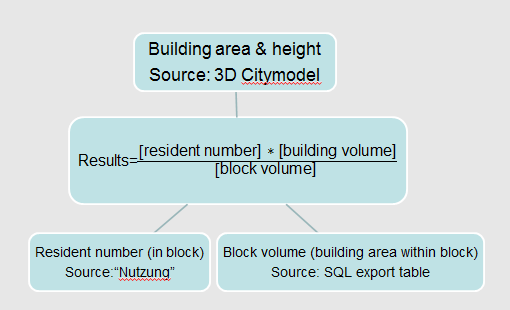
\includegraphics[width=0.8\textwidth]{phase1/group3/fig4.png}
	\caption{Inhabitants per Building (Self Made)}
	\label{fig:figure4}
\end{figure}


Figure \ref{fig:figure4} shows how to calculate the number of inhabitants in each building. In order to group the buildings per block, a spatial join is realized in ArcGis and the results are exported to the data-base. Then, as the buildings contain their “BlockId” attribute, as well as the sum of inhabitants in that block (for instance called “S” attribute), the residents shall be split into the buildings according to the next sentence:\\


$Ri= (Sk*Vi)/Vk$\\
\\
Where:\\
		Ri = Residents on building i\\
		Sk = Total number of inhabitants on block k\\
		Vi = Volume of building i\\
		Vk= Total Volume of buildings on block k

\subsection{Results}


Table 1 shows the results of Apartment/Volume for different building age group.

\begin{table}[ht]
	\centering
	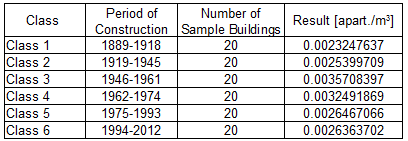
\includegraphics[width=0.8\textwidth]{phase1/group3/fig5.PNG}
	\caption{Indicator 'Apartments/Volume (m3)' (Self Made)}
	\label{fig:figure5}
\end{table}


\begin{figure}[ht]
	\centering
	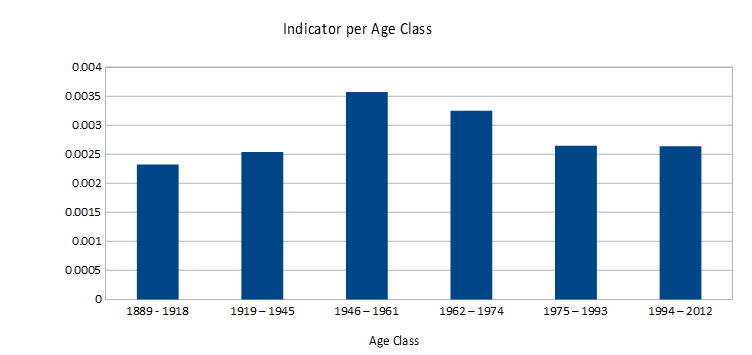
\includegraphics[width=0.8\textwidth]{phase1/group3/fig6.PNG}
	\caption{Indicators grouped by Age Class (Self Made)}
	\label{fig:figure6}
\end{figure}

Applying the indicators above, the apartment number for the whole test area can be calculated by multiplying the indicator with the building volume. Furthermore, the average household can by computed:\\
\begin{align}
Hi=\frac{Ri}{Ni}
\end{align}
Where:\\
H = Household average for building i\\
R = Total number of residents on building i\\
N = Number of apartments on building i (based on the volume)\\

The average result for the area of interest is: \textbf{H=1.584}
\\

As a validation procedure, the result might be compared to to statistical data on Figure 6. Statistically, the Mitte neighborhood presents 1.65 as household average value.

\begin{figure}[ht]
	\centering
	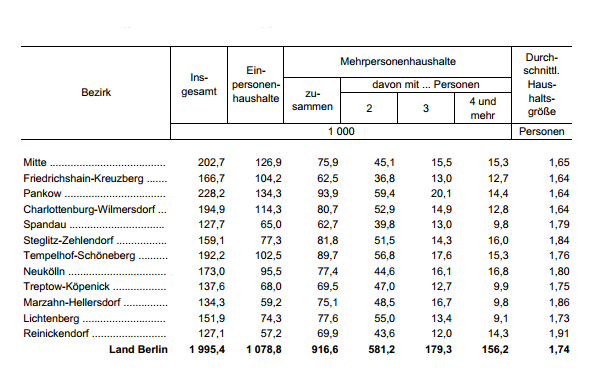
\includegraphics[width=0.8\textwidth]{phase1/group3/fig7.png}
	\caption{ Household in Berlin (Amt für Statistik Berlin-Brandenburg, 2011)}
	\label{fig:figure7}
\end{figure}


\part{Estimation of Energy Consumption and Energy Demand}
\newpage

\chapter{ %group 1
\section{Group1 - Calculation of buildings energy demand}
}
\subsection{Introduction}
The Task for the second phase was to calculate the building's energy demand using Java with the citygml4j library and the 3D city model. Necessary for that are the building’s volume and the attribution of walls as outer- or inner-/shared- wall surfaces which already was calculated by group one in phase one.\\
The most important information for this task are content of the so called IWU Report which is a report created by the IGG (Institute for Geodesy and Geoinformation Science) based on calculation methods of the "Institut Wohnen und Umwelt GmbH" [eng. Institute living and environment GmbH]. The IWU Report can be interpreted as a manual for the calculation of the building energy demand using the semantic citymodel of Berlin.\\
The document is structured into three parts: The determination of the input-values which are temperature, geometries and energy reference building-parameter, the calculation of the building's energy demand for space-heating using an accounting system and the calculation of the building's energy demand for warm-water.

\subsection{Input values}
For the calculation of energy flow of buildings, the surrounding climate is of an big importance. To take this into account some formulas contain a variable called "Gradstunden" which is representing the climate in a numerical value. For its calculation the summed up days per year have to be multiplied with the difference of the heated temperature inside and the actual temperature outside. To neglect the summer season in which buildings do not need any external heating energy, only the days with a switched on heater were considered.\\
The energy reference area is relevant for all calculations dealing with the building size. And due to the fact, that a precise indoor-model of the city is not available, the estimation of this value can be done with the formula (\ref{eq:energyReferenceArea}). Important to know is that only heated storeys without roof and cellar are taken into account.
\begin{equation}
	A_{EB} = 0.75 \times n_{G} x A_{FB} [m^2]
	\label{eq:energyReferenceArea}
\end{equation}
\begin{description}
	\item[$n_{G}$:] number of storeys
	\item[$A_{FB}$:] building footprint
\end{description}
Necessary for air-volume calculations inside, either the precise storey height have to known, or the average storey height which is depending on type and age of the building. Figure \ref{fig:storeyHeight} shows some average values of storey height depending on the building's age. Furthermore we took for our calculations additional 0.3m per storey in order to achieve (more or less) the same number of storeys as in real world. This number was found be supervising some samples of buildings which are part in our database-subset.
\begin{figure}[h]
	\centering
 	 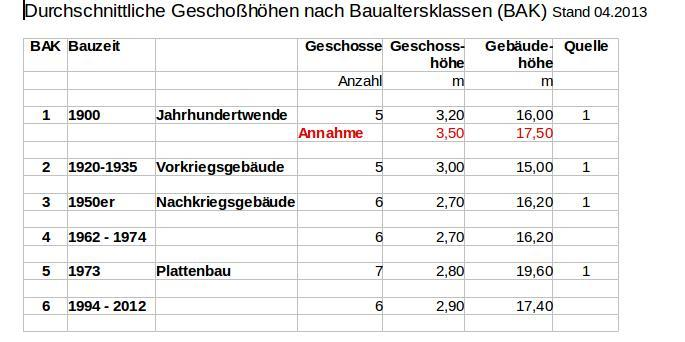
\includegraphics[scale=0.5]{phase2/group1/storey_height.jpg} 
	\caption{Average storey height depending on building's age. Provided by Michael Prytula.}
	 \label{fig:storeyHeight}
\end{figure}
The air-volume then can be calculated with the formula (\ref{eq:airVolume}) which is the energy reference area multiplied with the assumed mean (lighted) storey height.
\begin{equation}
	V_L = A_{EB} \times 2.5
	\label{eq:airVolume}
\end{equation}
Since some energy flows through building parts, its physical behaviour has be taken into account when calculation the energy flow. For this issue the so called U-values (in the IWU-Report called "k-Werte") are needed. They are describing the amount of energy transmitting between different building parts as for example between building-roof and building-main-part. Due to the fact that energy will not flow between two parts having the same temperature, it is important to know which wall surfaces are shared with also heating neighboured buildings. Figure \ref{fig:uValues} shows possible directions of the energy transmission, and possible building parts differentiated by its mean temperature. The afterwards following figure \ref{fig:uValuesTable} shows average U-values for specific building-ages and building-parts.
\begin{figure}[h]
	\centering
 	 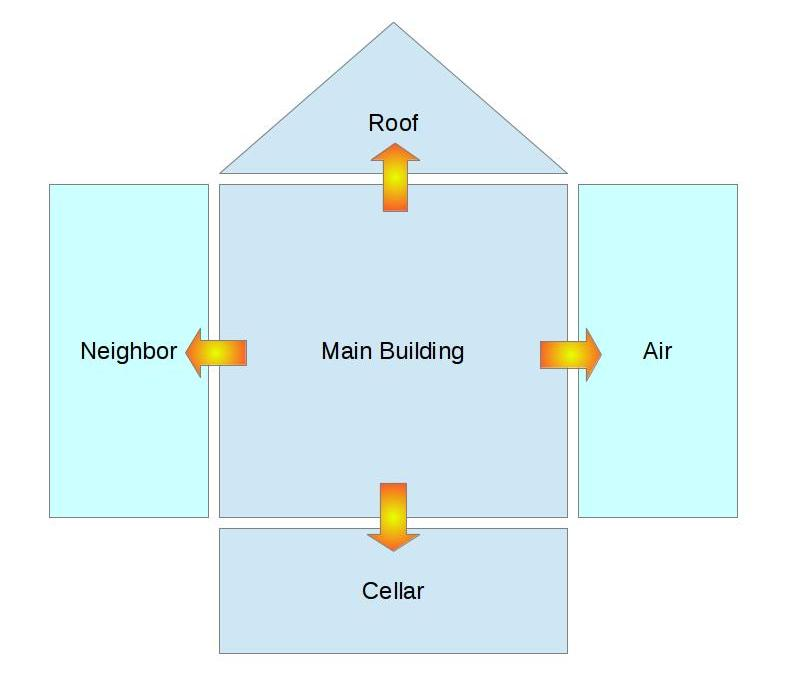
\includegraphics[scale=0.4]{phase2/group1/U-Values.jpg}
	\caption{Possible energy flow directions of a building.}
	\label{fig:uValues}
\end{figure}
\begin{figure}[h]
	\centering
 	 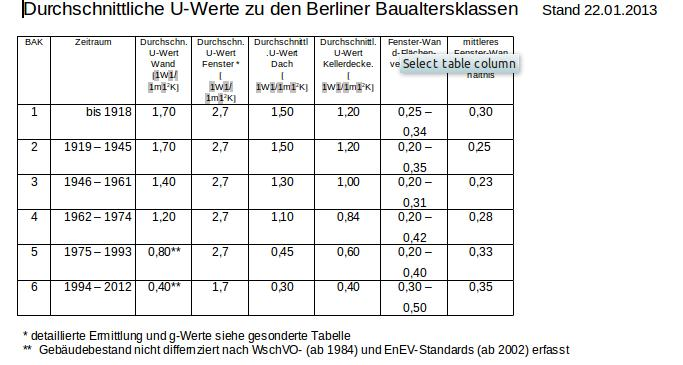
\includegraphics[scale=0.59]{phase2/group1/u-values_table.jpg}
	\caption{Average U-Values for specific building-ages and building-parts. Provided by Michael Prytula.}
	\label{fig:uValuesTable}
\end{figure}

\subsection{Demand of effective energy for heating}
The following formulas are describing the sequence of calculating the effective energy demand for heating. Later on following formulas are partially depending on the previous ones.\\
The calculation of the energy demand for heating can be easily done with using an accounting system as follows (\ref{eq:heatingDemand}):
\begin{equation}
Demand = Gain - Loss
\label{eq:heatingDemand}
\end{equation}
The Energy loss in [kWh/a] can be calculated as follows (\ref{eq:energyLoss}). 
\begin{equation}
Q_{V} = (Q_T + Q_L) \times f_{Abs}
\label{eq:energyLoss}
\end{equation}
\begin{description}
\item[$Q_{T}$:] transmission loss [kWh/a]
\item[$Q_L$: ]aeration loss [kWh/a]
\item[$f_{Abs}$:] reduction factor day-/night-setback
\end{description}
The values for the specific Day-nightsetback can be taken from a table with average values, depending on the building type (e.g. new-building).\\
The loss through transmission in [kWh/a] has to be taken from this formula (\ref{eq:lossTransmission}):
\begin{equation}
Q_T = (\sum f_i \times k_I \times A_i) \times \Theta 
\label{eq:lossTransmission}
\end{equation}
\begin{description}
\item[$f_i$:]reductionfactor [1.0 outer-walls; 0.5 inner-walls]
\item[$k_I$:] U-value [W/($m2$K)]
\item[$A_i$:] building's area [$m^2$]
\item[$\Theta$:] Gradstunden [kKh/a]
\end{description}
Summed up for every building part [i].\\
The loss through aeration in [kWh/a] can be calculated using the formula (\ref{eq:lossAeration}):
\begin{equation}
Q_L = 0.34 \times n \times V_L \times \Theta 
\label{eq:lossAeration}
\end{equation}
\begin{description}
\item[$n$:] frequency of aeration [1/h] (from table)
\item[$V_L$:] building's air volume [$m^3$]
\end{description}
For the energy gain following formulas have to be applied:\\
In general formula (\ref{eq:energyGain}) is describing the utilisation of the available free heat inside of the building:
\begin{equation}
Q_G = \eta_F \times Q_F 
\label{eq:energyGain}
\end{equation}
\begin{description}
\item[$\eta_F$:] utilisation
\item[$Q_F$:] free heat
\end{description}
The free heat is simply the solar irradiation plus the heat sources inside of the building (see formula (\ref{eq:freeHeat})).
\begin{equation}
Q_F = Q_S + Q_I 
\label{eq:freeHeat}
\end{equation}
\begin{description}
\item[$Q_S $:] solar irradiation
\item[$Q_I $:] heat sources inside
\end{description}
And following formula (\ref{eq:utilisation}) can be used for the utilisation:
\begin{equation}
\eta_F = 1 - 0.3 \times (\dfrac{Q_F}{Q_V}) 
\label{eq:utilisation}
\end{equation}
\begin{description}
\item[$Q_V $:] (remember:) energy-loss
\end{description}
As important income the solar energy gain can be calculated with the precise formula (\ref{eq:solarGain}) which needs precise knowledge about the window sizes.
\begin{equation}
Q_S = r \times g_{senkr} \times \sum G_i \times A_{F,i} 
\label{eq:solarGain}
\end{equation}
\begin{description}
\item[$G_i $:] global radiation per orientation (e.g. south)
\item[$A_{F,i} $:] window area per orientation [$m^2$]
\item[$g_{senkr} $:] energy transmission through glass-area (from Kurzverfahren Energieprofil)
\item[$r $:] reduction factor due to windows (standard value: 0.36)
\end{description}
Taking an factor for the window sizes per wall, also the following simplified formula (\ref{eq:simplySolarGain}) can be used for the calculations.
\begin{equation}
Q_S = r \times g_{senkr} \times 240 \times A_{window} 
\label{eq:simplySolarGain}
\end{equation}
\begin{description}
\item[$A_{window} $:] estimated overall window area [$m^2$]
\end{description}
Inside of buildings there are more heat sources than only the heater. For example electric devices like the light bulb are producing a lot of heat energy, which is also a factor for the calculations.\\
As a assumption, the next formula (\ref{eq:innerHeatSources}) is giving this factor a size.
\begin{equation}
Q_I = 0.024 \times q_i \times t_H \times A_{EB} 
\label{eq:innerHeatSources}
\end{equation}
\begin{description}
\item[$0.024 $:] factor for conversation ([W] $\rightarrow$ [kW]; [d] $\rightarrow$ [h]
\item[$q_i $:] specific power of inside heat sources [W/$m^2$]
\item[$t_H $:] heating period [d/a]
\item[$A_{EB} $:] energy reference area
\end{description}

\subsection{Demand of effective energy for warmwater}
The demand of warm water [kWh/a] can more easily be calculated. It is simply the demand per person multiplied with the number of persons living in the building. The formula (\ref{eq:warmWater}) shows how this can be calculated.
\begin{equation}
Q_W = \dfrac{Q_{W/P} \times A_{EB}}{A_{EB/P}}
\label{eq:warmWater}
\end{equation}
\begin{description}
\item[$Q_{W/P} $:] demand of warm water per year and person [kWh/(P a)] (standard: 600 kWh/(P a))\\
\item[$A_{EB/P} $:] living space per person [$m^2$/P] (standard: 35 $m^2$/P)\\
\end{description}
This formula calculates the number of persons living in the building by dividing the energy related area by the average space per person. When having a more precise estimation of inhabitants per building as group three was calculating, the formula can be changed into the formula (\ref{eq:simplyWarmWater}):
\begin{equation}
Q_W = Q_{W/P} \times N_P
\label{eq:simplyWarmWater}
\end{equation}
\begin{description}
\item[$N_P$:] number of persons\\
\end{description}

\subsection{Result}
As results of the calculations, the Java algorithm produces a .csv file containing information about each building which has an own identifier. All values are calculated in [kWh/a]. The table shows a subset of the result file, with three buildings and the interesting attributes described in this report.
\begin{table}[b]
\centering
\begin{tabular}{c  c  c  c  c  c}
building\_id & heating\_loss & heating\_gain & ... & ..demand\_heating & ..demand\_warmwater \\
\hline						
BLDG\_000300000026ed79 & 116670,763	& 15572,718 & ... & 101098,045 & 4805,405\\
BLDG\_000300000026f491 & 229314,037	& 32343,216 & ... & 196970,821 & 16289,207\\
BLDG\_000300000026f4a7 & 216882,225	& 31687,923 & ... & 185194,302 & 15044,102\\
...\\
\end{tabular}
\label{table:result IWU-Report}
\caption{Results of the IWU-report-calculation [kWh/a].} 
\end{table}

\subsection{Discussion}
The number of storeys is one central value of all calculation, because with a wrong estimated number of storeys the reference are can change rapidly. Figure \ref{fig:changeArea} shows how the reference area is changing with the wrong estimated number of storeys.
\begin{figure}[h]
	\centering
 	 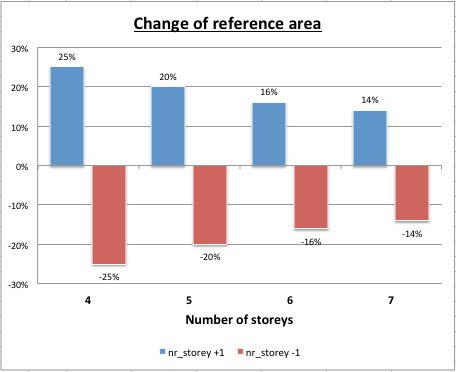
\includegraphics[scale=0.5]{phase2/group1/change_area.png} 
	\caption{Changing area with wrong estimated number of storeys.}
	 \label{fig:changeArea}
\end{figure}
And therewith also the calculated energy parameters which are depending on the reference area are changing.  Figure \ref{fig:changeParameter} shows how strong they are depending on a right estimated number of storeys.
\begin{figure}[h]
	\centering
 	 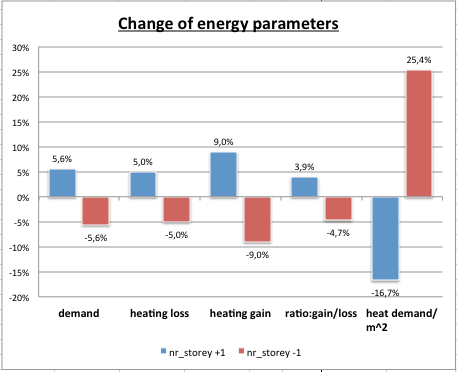
\includegraphics[scale=0.5]{phase2/group1/change_param.png} 
	\caption{Changing energy parameters with wrong estimated number of storeys.}
	 \label{fig:changeParameter}
\end{figure}

Following improvements could be helpful to obtain better results:\\
First as mentioned before we took additional 0.3m to obtain a better estimation, this is because in the calculations the average storey height was describing the inside storey height without ceiling thickness.\\
Maybe it would be useful to consider the building's usage for the estimation of the specific storey height.\\
In the IWU report 2.5m were assumed as the storey height for the air-volume, in our calculations we were using the previously calculated storey height.


\newpage

\chapter{ %group 2
\section{Group 2 - Estimation of the Solar Potential}
}
%%**************************************************************
%% GIS project report
%%**************************************************************

% possible structure
% x Estimation of the solar Potential with 3D CityDB (Introduction) DONE
% x.2 Workflow (Steffen) DONE
% x.3 Basics of PV systems (Hannah)DONE
% x.4 Basics of ST systems (Steffen) DONE
% x.5 Solar irradiance (Hannah) DONE
% 	x.5.1 Tilt (Hannah) DONE
% 	x.5.2 azimuth (Hannah) DONE
% 	x.5.3 satel light db (Hannah) DONE
% x.6 Roof surface area DONE
% 	x.6.1 simple reduction (Steffen) DONE
% 	x.6.2 reduction due to building age classes (Steffen) DONE
% x.7 Shadowing (Steffen) DONE
% x.8 Calculation of the potential DONE
%	x.8.1 Photovoltaic (Hannah) DONE
% 	x.8.2 Solar Thermal (Steffen) DONE
% x.9 Results (Steffen)
%	x.9.1 Test Area (Steffen)
% 	x.9.2 Validation (Steffen)
% x.10 Visualization (Hannah)
% x.11 Conclusion (Hannah) First version is DONE
% x.12 Future Work (Hannah) DONE


%\documentclass[10pt,a4paper,portrait]{article}
\usepackage{geometry}                % See geometry.pdf to learn the layout options. There are lots.
\geometry{a4paper}                   % ... or a4paper or a5paper or ... 
%\geometry{landscape}                % Activate for for rotated page geometry
\usepackage[parfill]{parskip}    % Activate to begin paragraphs with an empty line rather than an indent
\usepackage{graphicx}
\usepackage{subfig}
\usepackage{amssymb}
\usepackage{amsmath}
\usepackage{epstopdf}
\usepackage{multicol}
\usepackage{amsmath}
\usepackage{listings}
\usepackage{url}
\usepackage{multirow}
\usepackage{color}
\definecolor{grey}{rgb}{0.5,0.5,0.5}
\definecolor{darkgreen}{rgb}{0.5,0.5,0.0}
\lstset{ %
language=Matlab, % the language of the code
basicstyle=\ttfamily, % the size of the fonts
       % that are used for the code
numbers=left, % where to put the line-numbers
numberstyle=\footnotesize, % the size of the
        %fonts that are used for the line-numbers
stepnumber=1, % the step between two
       % line-numbers. If it's 1, each line 
keywordstyle=\color{darkgreen}, % Keywords
       % font ('*' = uppercase)
commentstyle=\color{grey},
numbersep=5pt, % how far the line-numbers are
       % from the code
backgroundcolor=\color{white}, % choose the
        %background color. You must add \usepackage{color}
showspaces=false, % show spaces adding
        %particular underscores
showstringspaces=false, % underline spaces
        %within strings
showtabs=false, % show tabs within strings
       % adding particular underscores
frame=single, % adds a frame around the code
tabsize=2, % sets default tabsize to 2 spaces
captionpos=b, % sets the caption-position to
        %bottom
breaklines=true, % sets automatic line
        %breaking
breakatwhitespace=false, % sets if automatic
        %breaks should only happen at whitespace
 % show the filename of files included with
       % \lstinputlisting;
 % also try caption instead of title
escapeinside={\%*}{*)} % if you want to add a
       % comment within your code
}
\DeclareGraphicsRule{.tif}{png}{.png}{`convert #1 `dirname #1`/`basename #1 .tif`.png}
% 
% \begin{document}
% 
% % Titlepage with task representation
% \input{include/title}	
% \newpage
% 	

% Introduction + workflow
-This chapter will describe how the system will be designed, how the Field of application can be modelled, what functionalities can be planned-

\section{Einsatzgebiet}
Um präzise beschreiben zu können was das System tun können muss, ist es notwendig vorher konkret die vorliegende Situation oder das existierende Problem zu definieren. Solche eine Definition sollte eine Beschreibung der Umgebung beinhalten in der das System eingesetzt werden soll. Nimmt man eine Modellierungssprache zur Hilfe, um die Umgebung zu beschrieben, ist es später einfacher daraus Rückschlüsse auf mögliche Probleme zu ziehen. Für ein solches Modell müssen die Fragen beantwortet werden, in welche Objekte sich die Umgebung aufgliedert, wie diese interagieren und welche Funktionalitäten diese dafür verwenden.Aber auch die teilhabenden Akteure und ihre konkreten Anforderungen an das System müssen modelliert werden. Mit Hilfe von exemplarischen Anwendungsfällen werde ich beschreiben was der tatsächliche Bedarf des Nutzers ist, und wie dieser gedeckt werden kann.

Bevor ich mit dem technischen Ausformulieren der Modellierung beginne, möchte ich kurz in die Thematik einleiten: Das System welches ich mit dieser Arbeit konzeptioniere soll Feldingenieuren helfen im Feld mit den Messungen und Daten verschiedener Sensoren zu arbeiten. Als konkretes Beispiel werde ich den Einsatz des Systems bei der Bauwerksüberwachung mithilfe eines Sensornetzwerkes beschreiben.

Die Überwachung von Bauwerken mittels eines Netzwerkes aus verschiedenen Sensoren hilft ihre Sicherheit ohne den Einsatz großer Bautechnischer Überprüfungen einschätzen zu können. Damit ist es möglich Bauwerke auch weit über ihre geplante Lebensdauer hinweg zu erhalten. Ohne den Einsatz solcher Sensor Netzwerke können die zuständigen Gutachter bei Ablauf der geplanten Lebensdauer nicht darauf vertrauen, dass das Gebäude auch weiterhin den kontinuierlichen Belastungen gewachsen ist, und somit werden entweder umfangreiche Sanierungen Nötig, oder Gebäude werde geschlossen. Die Überwachung basiert auf der Messung von Veränderungen von verschiedenen Parametern wie zum Beispiel der Position , der Temperatur oder Feuchtigkeit von Bauteile oder der Abweichungen von charakteristischen Bewegungsmustern von Bauteilen, gemessen durch Beschleunigungssensoren. Die Parameter werden sowohl punktuell  verteilt über das gesamt Bauwerk, als auch gesamtheitlich die Struktur des Bauwerkes miteinbeziehend erhoben, siehe auch \citep{worden_overview_2004} \citep{farrar_introduction_2007} \citep{boller_structural_2004}. Für die Messungen werden zum einen automatisch kontinuierlich messende Systeme eingesetzt, und zum anderen seltenere manuelle Messungen, deren Ergebnisse manuelle in das System eingegeben werden. 

Für das bessere Verständnis möchte ich hier ein Beispielfall beschreiben: Ein Brücke erreicht ihre letzten Jahre der Betriebserlaubnis. Danach müssen entweder die Verkehrssicherheit erneut umfangreich geprüft, und zahlreiche Verschleißteile, deren Zustand schlecht zu beurteilen ist, ersetzt werden, oder die Verkehrssicherheit muss auf andere Art überprüft werden. Zahlreiche Sensoren werden an den einzelnen wichtigen Gebäudeteilen eingerichtet, und überwachen nun automatisch über einen bestimmten Zeitraum deren Verhalten und Veränderungen. In periodischen Abständen werden automatisch Diagnosen erstellt, basierend auf der Analyse der Messwerte, der Überprüfung des Materialverschleißes und einiger anderer Einflussgrößen. Eine detailliertere Beschreibung der verwendeten Messungen, Zeitskalen und Analysemethoden werden in den nachfolgenden Kapiteln beschrieben.

In der Einleitung der Arbeit möchte ich mich am Verlauf der Erstellung eines Pflichtenheftes für die Softwareentwicklung orientieren , da so am besten modelliert werden kann wie der Bedarf des Nutzers gedeckt werden kann, siehe auch \citep{gregor_engels_vorlesung_2006}. Beginnen werde ich mit einer textuellen Beschreibung der Situation. Danach folgt eine Modellierung der Prozesse und der Akteure mit ihren jeweiligen Anwendungsfällen. Zum Abschluss werde ich dann die daraus abgeleiteten notwendigen Funktionalitäten des System beschreiben.


\subsection{Modell des Problembereichs}
Die Abbildung \ref{fig:model_domain} zeigt ein UML Diagramm (Unified Modeling Language) das die im folgenden beschrieben verschiedenen Objekte des Systems beinhaltet. Das Modell beschreibt die Beziehungen der einzelnen Objekte untereinander und modelliert keine Aktivitäten oder Funktionen.

Die Umgebung in der das System eingesetzt werden wird besteht aus fünf verschiedenen Arten von Objekten und deren Beziehungen untereinander. Zentrales Objekt ist der Daten Server, der als Knoten für die Kommunikation zwischen den einzelnen Kompartimente dient. Diese sind hauptsächlich die Sensoren selbst, die jedoch ohne einen Server, der als Steuerungseinheit für jeden Sensor dient, nicht selbständig messen können. Der Server kontrolliert die Sensoren indem er sie aktiviert und deaktiviert. Nichtsdestotrotz können Sensoren in einem separiertem eigenem Netzwerk organisiert sein, das dann wiederum als einzelner Sensor behandelt wird. Die Sensoren senden ihre gemessenen Daten entweder aktiv an den Server beziehungsweise über den Server an die dem Server angeschlossene Datenbank, oder der Server ruft die Daten aktiv ab, und speichert diese dann in der Datenbank.

\begin{figure}[H]
	\centering
 	 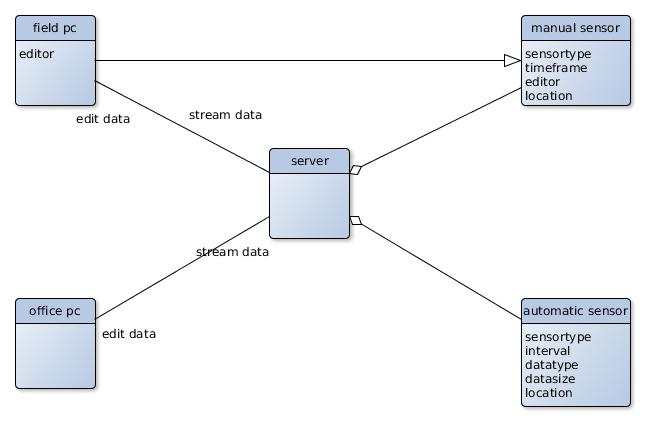
\includegraphics[scale=0.6]{graphics/model_of_issue.jpg} 
	\caption{Modell des Problembereiches mit relevanten Objekten, F. H. Euteneuer 2013}
	 \label{fig:model_domain}
\end{figure}

Die Datenbank die and den Server angeschlossen ist speichert sowohl Metadaten zu den Sensoren, als auch die gemessenen Werte. Unter Metadaten sind alle Informationen zu verstehen, die die Sensoren eindeutig beschreiben, und die für weitere Analysen der Messerwerte erforderlich sind (siehe auch im Glossar "Metadaten". Beispielsweise sind das die Positionen der Sensoren, die Messintervalle, die Sensortypen oder die übermittelten Datentypen.

Als Klient des Services kann im Prinzip jede Art von mobilen Systemen eingesetzt werden. Angeschlossen an die Datenbank dienen diese dann als bildgebender Teil des Systems. Da die Verknüpfung mit einem Server meist über das Protokoll TCP/IP geschieht, müssen mobile Geräte über eine Internetverbindung verfügen. Die Verwendung dieser Geräte bleibt dadurch begrenzt auf Gebiete innerhalb der Handynetz-Abdeckung. Für manuelle Messungen dient der mobile Klient zusätzlich als Eingabegerät für die Messwerte, sofern dies nicht über das Gerät selber erfolgen kann. Dadurch wird der mobile Klient in dem Modell sowohl als bildgebender Teil des Systems, als auch als Sensor behandelt, und ererbt damit die Eigenschaften des Sensor Objekts.

Das System will einen ganzheitlichen Ansatz verfolgen, und beinhaltet somit auch einen Teil der für die umfangreicheren Analysen zuständig ist, sowie durch eine Datenexportfunktion als Schnittstelle zu weiteren Algorithmen und System dient. Dieser Teil des System wird in dem Modell durch den "Desktop-Computer" repräsentiert. Die eigentliche Einrichtung und Planung des Systems wird erwartungsgemäß von diesem, dem bequemeren Arbeitsplatz (verglichen mit dem mobilen Klienten), durchgeführt werden. Zusätzlich zu den Eigenschaften des Feldcomputers sind somit erweiterte Verwaltungs- und Analysefunktionen als Eigenschaften dieses Objektes definiert.


\subsection{Geschäftsprozesse}
Wichtigste Entscheidungshilfe für die Nutzung solch eines Systems wird die Eigenschaft des Systems, eine entscheidungsunterstützende Funktion zu erfüllen, sein. Das System ist fokussiert auf die wichtigen Werkzeuge die die Arbeit des Feldingenieurs vereinfachen sollen, und lässt unwichtige oder komplizierte Werkzeuge komplett weg. Außerdem werden die Informationen die im Feld auf dem mobilen Klienten angezeigt werden derart reduziert, dass lediglich aussagekräftige Werte, die damit Entscheidungen unterstützen können, angezeigt werden. In dem vorherigem Kapitel habe ich den Problembereich beschrieben, nun möchte ich die verschiedenen Prozesse skizzieren die ein Nutzer durchführen könnte.

\begin{figure}[H]
	\centering
 	 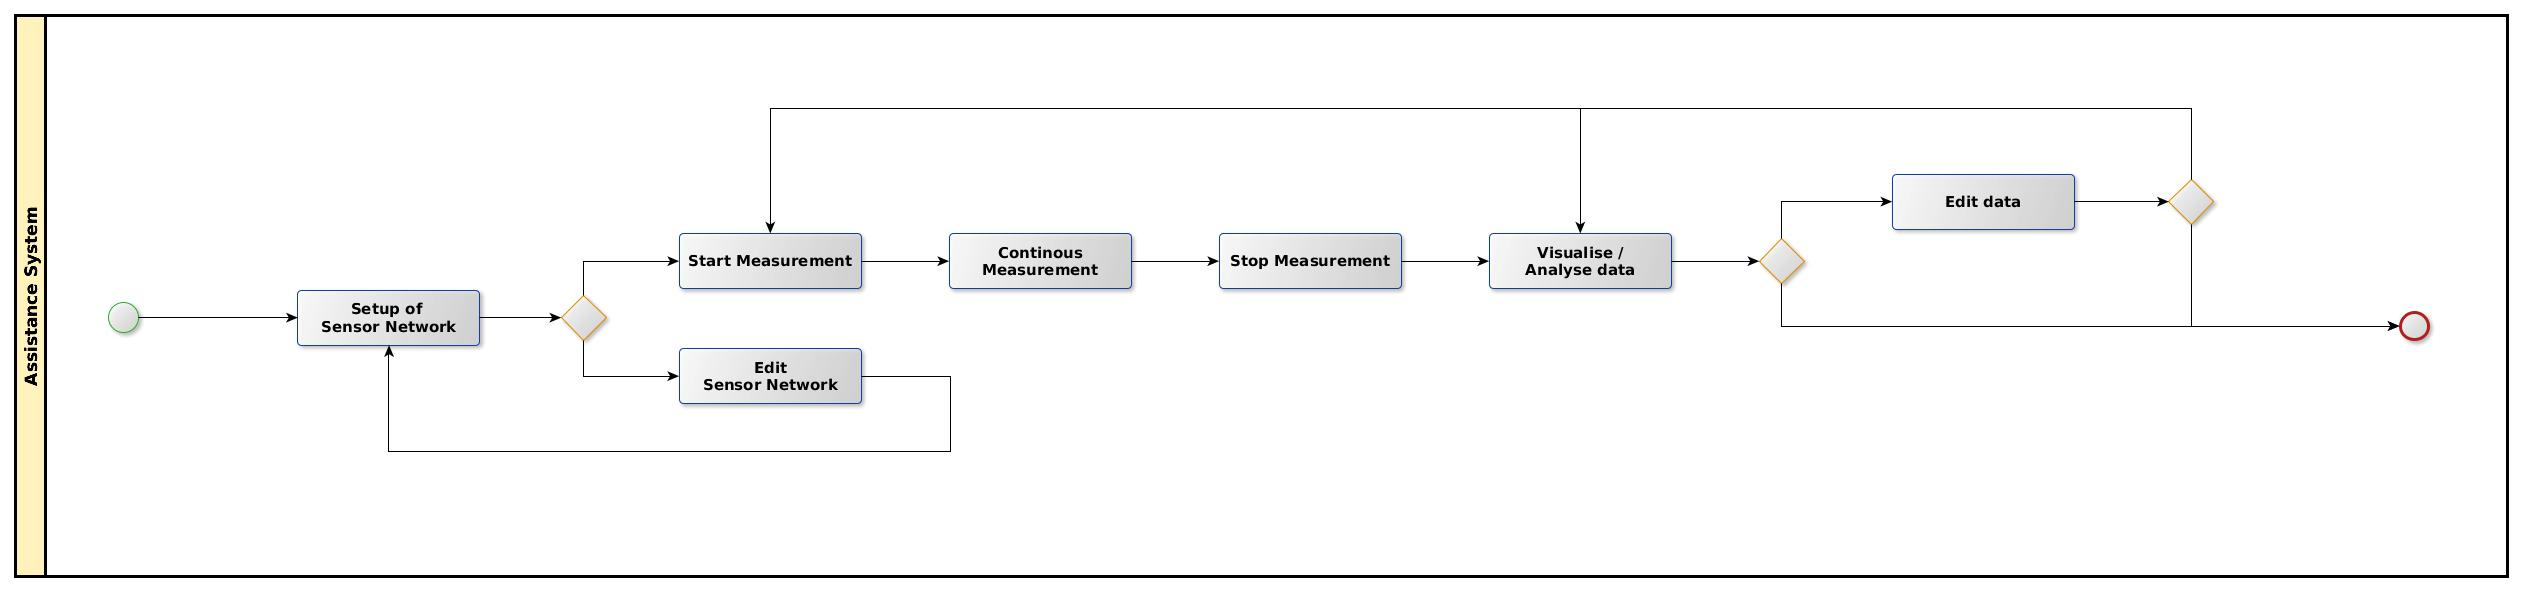
\includegraphics[scale=0.2]{graphics/bpmn_business-processes.jpg} 
	\caption{BPMN (Business Process Model and Notation) Modell relevanter Aktionen welche in dem System durchgeführt werden, F. H. Euteneuer 2013}
	 \label{fig:model_business-processes}
\end{figure}

Ich habe drei verschiedene Hauptaktionen identifiziert, die ein Nutzer durchführen könnte: Das manuelle Messen von Werten, das manuelle Editieren bereits gemessener Werte, und das automatische kontinuierliche Messen. Die Abbildung \ref{fig:model_business-processes} veranschaulicht mittels eines UML Activity Diagrams (UML Aktivitäten Diagramm) die einzelnen Abläufe dieser Aktionen.

Die manuelle Messung beginnt mir der normalen Messung der Werte. Im zweiten Schritt erfolgt die Eingabe der Werte in das System. Die Werte werden automatisch auf ihre Validität hin überprüft, und erste einfache statistische Analysen werden erstellt. Diese erste Statistik ist erforderlich um Informationen über die Qualität der Messung zu erhalten, und dem System die Möglichkeit zu bieten fehlerhafte Messungen zu bemängeln und Neumessungen vorzuschlagen.

Der Nutzer wird die Möglichkeit haben vergangene Messungen manuell zu bearbeiten. Dazu muss ein Datensatz (Üblicherweise ein Messwert) ausgewählt werden, und der Nutzer kann dann entscheiden ob die betreffende Messung wiederholt werden soll, oder die Werte manuell geändert werden sollen. Bei einer Wiederholung der Messung wird die Prozesskette der manuellen Messung durchlaufen.


The automatic measurements are the most important one for the described SHM. The will be the backbone of the system, nevertheless they are using similar functionalities. The user will initially be able to set the sensor network up. Which means to enter metadata about the used sensors like position, reference system, type of sensor, measurement interval, etc. A more detailed description of what is needed for such a setup will follow in the methodical part. After the setup, the user is able to start the measurements with the defined parameter, or the edit the settings.

As a conclusion of this chapter, I would like to point out that this list is only representing functionalities of a basic system, and should not be understood as being complete.


\section{Functionalities}
This chapter will describe what the system should provide to solve the problem and/or make the existing situation better: Which functionalities should be part of the system. To get closer to a possible solution, the different stakeholders and their use cases in the domain of structural health monitoring must be defined and described.

\begin{figure}[H]
	\centering
 	 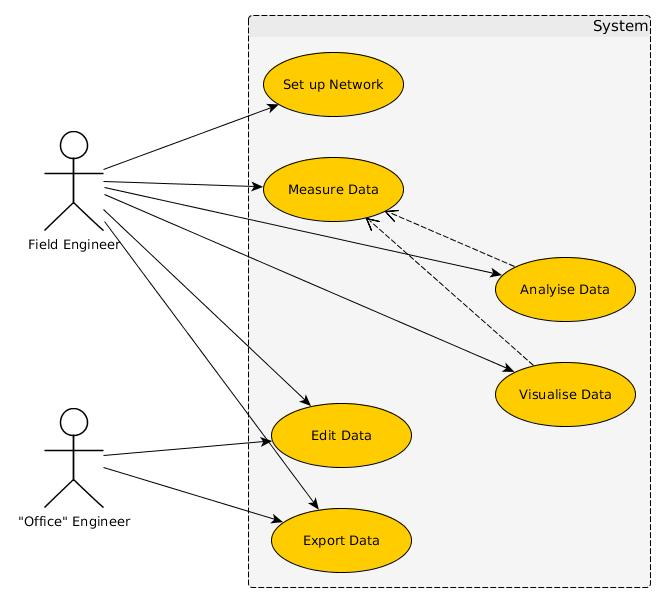
\includegraphics[scale=0.6]{graphics/uml_functionalities.jpg} 
	\caption{UML Use Case Diagram of the described System describing two different users and their use cases. By F. H. Euteneuer 2013}
	 \label{fig:model_functionalities}
\end{figure}

\subsection{Usergroups}
As a main source for information and parameter for the concept of a software, the usergroups are of large importance. I will analyse the involved usergroups and their needs respective expectations to get those information. As the figure \ref{fig:model_functionalities} is already representing, I have identified two main usergroups which might be involved in the processes.

\subsubsection{Field-engineer}
The group of field-engineers can described as the executive persons which are dealing with the direct measurements, observations and setup of an automatic measurement network. This group can be categorised by its technically limits, which are:
\begin{itemize}
\item the small screen-size of the mobile computers (quality of visualisation is limited)
\item the lack of input facilities (e.g. only digital keyboard on a handheld computer)
\item high weight of not handheld instruments (e.g. a conventional laptops too heavy for using while walking/standing)
\end{itemize}
But nevertheless, this usergroup has the most challenging requirements on the system when speaking about visualisation options or analysis computation in advance. It is the central target usergroup for this system, therefore it should fit mostly to its requirements.


\subsubsection{Office-engineer}
Usually the field-engineer and the office-engineer are combined in one person. One part of an observation project is dealing with the field-work, the setup, measurements and maintenance. And the other part is the precise analysis of the data, the post processing and its interpretation. Due to a high quality equipment in the offices, this part is mostly better solvable for a software. Here does not the system has to be restricted by the environment, but the system is making its demands on the technical environment.


\subsection{Use Cases}
The Figure \ref{fig:model_functionalities} is showing the different basic use cases of the described two usergroups. Use cases shown in this figure are representing activities of the user which have to be complete with it own defined target. I want now describe the use cases in detail with further parameter. This is important for the further proceeding of the system conception, because use cases are defining the users interests of a system.

The following part will describe the selected use cases in detail. All the use cases will be described with tables for the textual description which are containing information about the use case goal, the postcondition and further more. For the description of the the chronological task flow of the use cases also a activity diagram will depict each use case.

Important to know is, that the diagrams are not representing all possible activity flows which are available. They are representing one possible option which could solve the problem and will be implemented in the prototype.

The use cases are divided into three different groups. There are use cases dealing with central data management functionalities, others are describing main measurement functionalities and the last are describing the data analysis functionalities.


\subsubsection{Management}
There are several use cases with central management functionalities of the system. Management stands for both, data management and system management.  

First use case within the system is the setting up of the network. It can be understood as the initial task and therefore a kind of a precondition for all other use cases.The table \ref{table:use case description of "Set up network"} is describing central features of this use case. 

The export of the data is another major task within the management field. It could be denoted as the final task interacting with the system. The second table \ref{table:use case description of "Export data"} is showing detailed information about the "Export data" use case.

\begin{table}[H]
\centering
\begin{tabular}{l | p{11cm}}
Name & Set up network\\ \hline 
Usergroup & Field engineer\\ \hline 
Goal & Input all metadata about connected sensors and initialise network\\ \hline 
Precondition & Network physically existing and able to correspond with system\\ \hline 
Postcondition & working network with all sensors\\ 
\end{tabular}
\caption{Use Cases tabular description of characteristics} 
\label{table:use case description of "Set up network"}
\end{table}

\begin{table}[H]
\centering
\begin{tabular}{l | p{11cm}}
Name & Export data\\ \hline 
Usergroup & Office Engineer\\ \hline 
Goal & Specify data by parameter and specify output format\\ \hline 
Precondition & Specified data and output format\\ \hline 
Postcondition & complete dataset in specific format offline\\ 
\end{tabular}
\caption{Use Cases tabular description of characteristics} 
\label{table:use case description of "Export data"}
\end{table}

Figure \ref{fig:bpmn_use-case_management} is showing the systems management use cases in a two line activity diagram. The both activity flows do not have any interaction in between, but chronologically must the setup use case performed before the export use case.

The activity flow of the setup use case is showing two main tasks: The database-setup and the input of the sensor-parameter. Those are the central parts and their success or failure is leading to an overall success or failure. An edit of an existing network is leading to a restart of the full procedure. This could be interpreted as an assistant which is leading through the different configurations and is taking care of possible errors.

The export use case is much easier, it is simply the normal flow which is equal to most of the download assistants which can be found online. The only important information about that is the determination of the export datasets time-frame.

\begin{figure}[H]
	\centering
 	 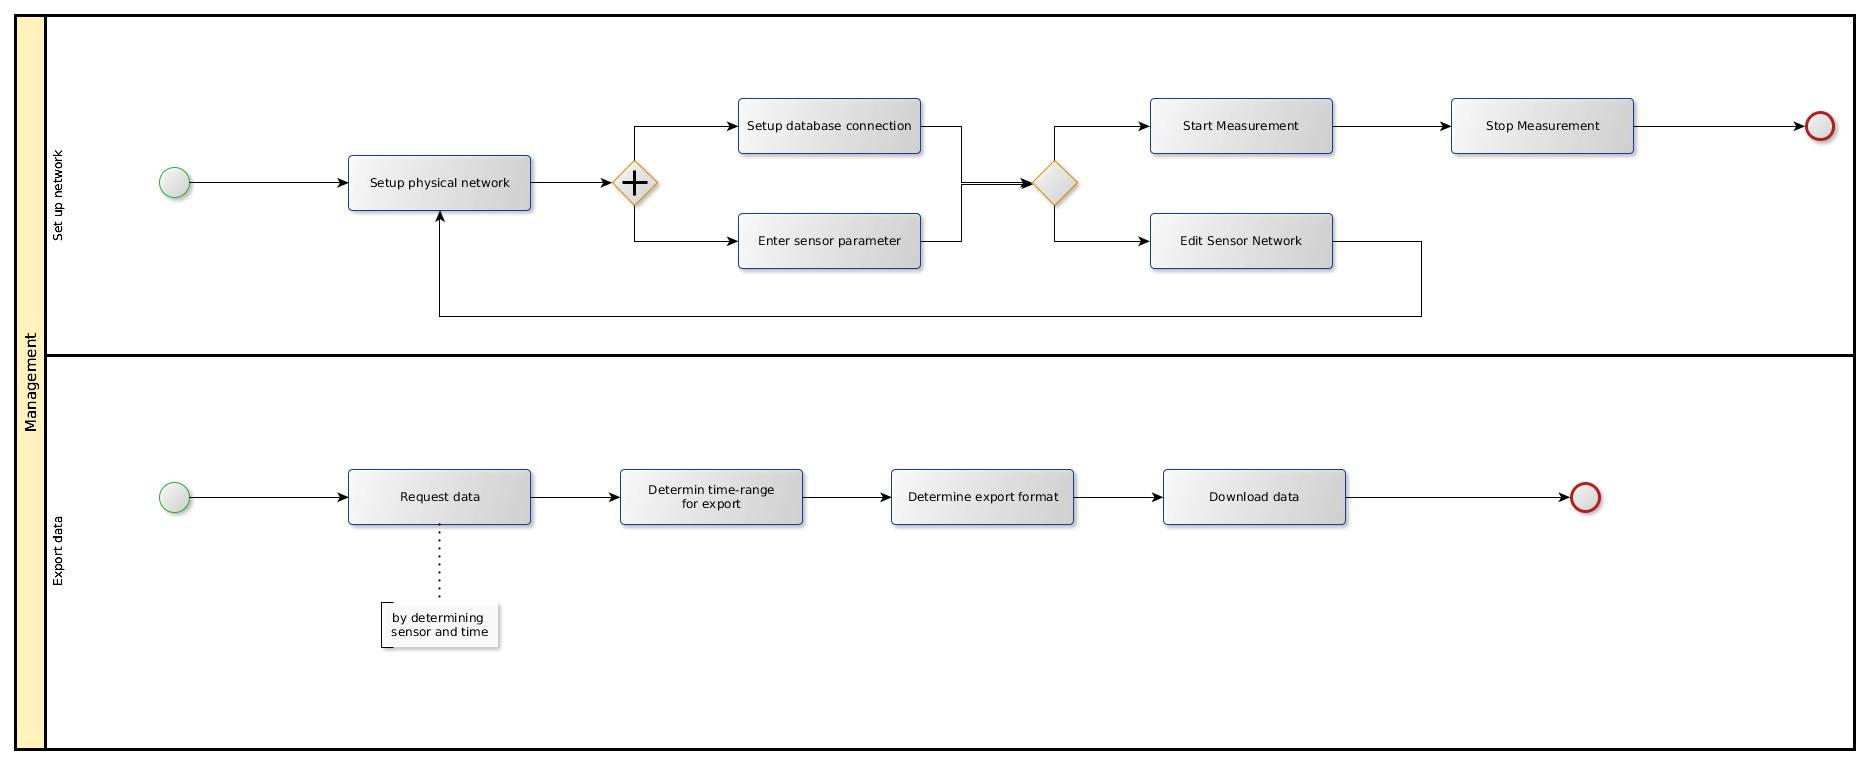
\includegraphics[scale=0.24]{graphics/bpmn_use-cases_management.jpg} 
	\caption{BPMN (Business Process Model and Notation) Model of the use cases describing central management proceedings. By F. H. Euteneuer 2013}
	 \label{fig:bpmn_use-case_management}
\end{figure}


\subsubsection{Measuring}

The measurement part might be the most important one within the system. This part is the only one which is describing a manual manipulation of the data in the database.

There are two identified use cases: The first is dealing with the initial data input which is the measurement see table \ref{table:use case description of "Measure data"}. In contrast to the automatic measurements, this is describing a discrete manual measurement, and the input of the data by hand.

And the second one is editing already existing data in the database see table \ref{table:use case description of "Edit data"}. This is a merely a standard operation for database related systems. Nevertheless, this task is related to the measurement task, in case of re-measuring data or validation of data.

\begin{table}[H]
\centering
\begin{tabular}{l | p{11cm}}
Name & Measure data\\ \hline 
Usergroup & Field engineer\\ \hline 
Goal & Input all data by hand  getting from standalone measurement device\\ \hline 
Precondition & Running system and access to database\\ \hline 
Postcondition & valid data in the database with full set of metadata\\ 
\end{tabular}
\caption{Use Cases tabular description of characteristics} 
\label{table:use case description of "Measure data"}
\end{table}

\begin{table}[H]
\centering
\begin{tabular}{l | p{11cm}}
Name & Edit data\\ \hline 
Usergroup & Office Engineer\\ \hline 
Goal & Specify data by parameter and input new values by hand or measurement\\ \hline 
Precondition & Running system and access to database\\ \hline 
Postcondition & changed data in the database with full set of metadata\\ 
\end{tabular}
\caption{Use Cases tabular description of characteristics} 
\label{table:use case description of "Edit data"}
\end{table}

When performing a manual measurement, most of the task described in the first line of the figure \ref{fig:bpmn_use-case_measuring} will be mandatory tasks. In the end the system will perform a quick analysis of the inserted data in order to validate the measurement. After this step the system will either point out possible errors, or it will approve the measurements, and write them into the database. The second line, the editing flow, is offering two options, one is a manual insert of new data, another would lead to a re-entering of the manual measurement flow, in order to overwrite the selected datasets with new measurements.

\begin{figure}[H]
	\centering
 	 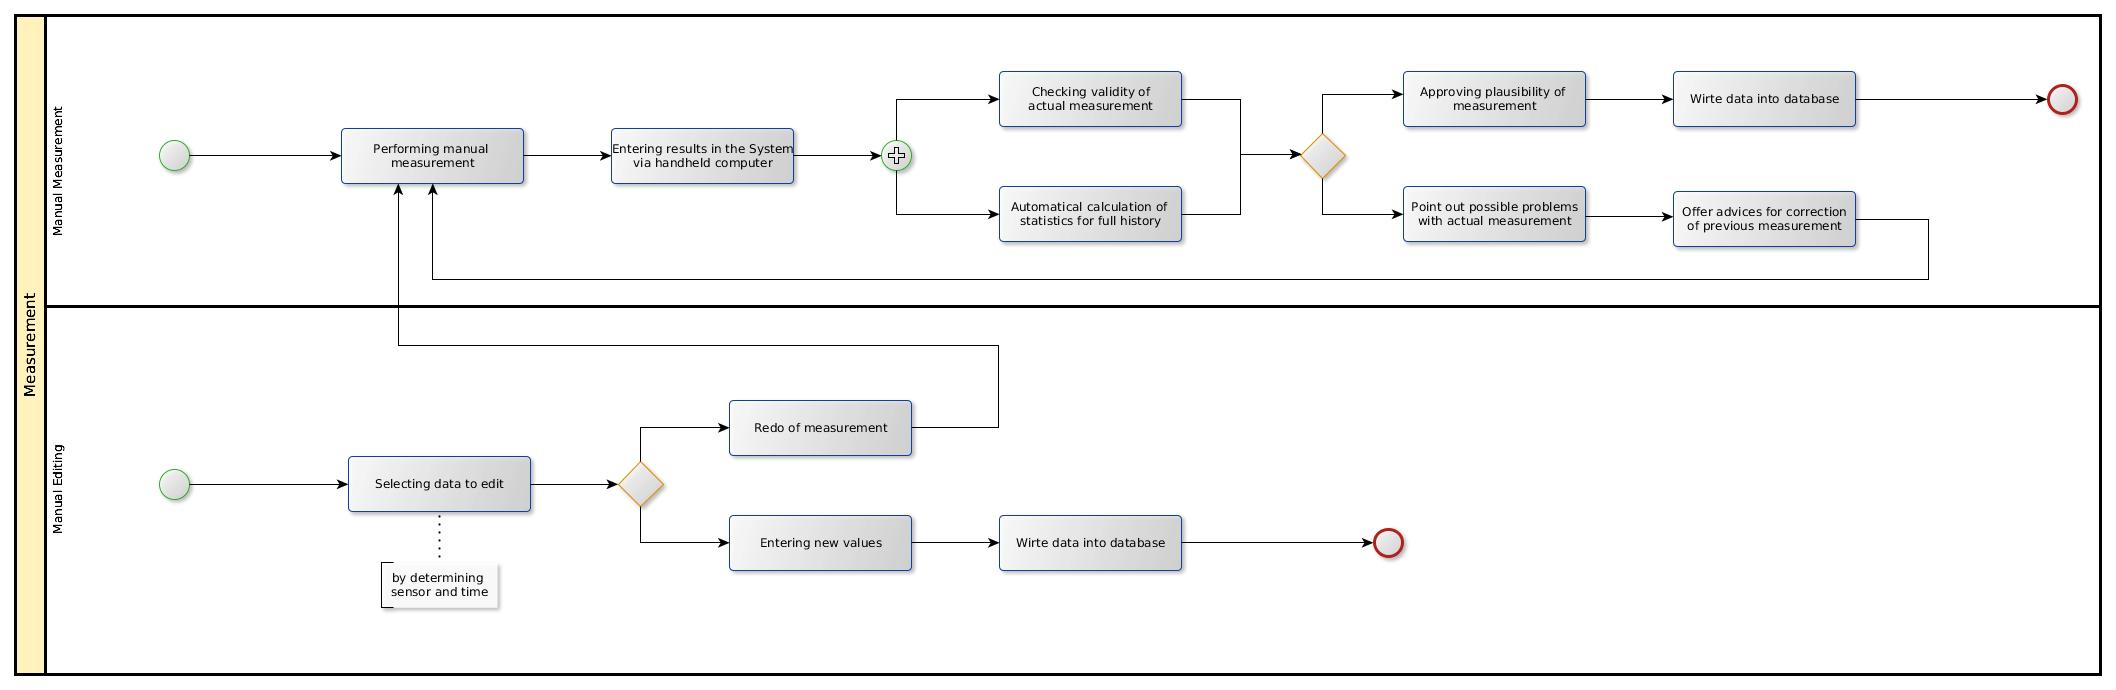
\includegraphics[scale=0.24]{graphics/bpmn_use-cases_measurement.jpg} 
	\caption{BPMN (Business Process Model and Notation) Model of the use cases describing central measuring proceedings. By F. H. Euteneuer 2013}
	 \label{fig:bpmn_use-case_measuring}
\end{figure}

\subsubsection{Analysis}

A complex part is the analysis functionalities of the system which will be described in this section. The analysis described here will be slightly different to the "ad hoc" statistics in the previous part which are leading to approved or discarded measurements. Those are checking the coherence of the performed measurements. The analysis described here are producing also easy and quick statistics, but in comparison to historical data see table \ref{table:use case description of "Analyse data"}. The user will be able to recheck if the measurements are leading to similar results, or if the measurements are possibly done with wrong parameters. 

The other analysis part is a visual analysis of the data (see table \ref{table:use case description "Visualise data"}). The system will here produce some graphics representing the measurement, the observed object and the related statistics. An optical validation of the performed measurements, and additionally to that, an optical representation of real-time data is a big advantage for the field-engineer (as described in the overall introduction).

\begin{table}[H]
\centering
\begin{tabular}{l | p{11cm}}
Name & Visualise data\\ \hline 
Usergroup & Field engineer\\ \hline 
Goal & Getting support by visualising measurements and interpretation\\ \hline 
Precondition & Existing meatadata for measurements\\ \hline 
Postcondition & meaningful and „supporting“ graphic\\
\end{tabular}
\caption{Use Cases tabular description of characteristics} 
\label{table:use case description "Visualise data"}
\end{table}

\begin{table}[H]
\centering
\begin{tabular}{l | p{11cm}}
Name & Analyse data\\ \hline 
Usergroup & Field engineer\\ \hline 
Goal & Getting information about validity of data in comparison to historical data\\ \hline 
Precondition & Amount of measurements higher then two\\ \hline 
Postcondition & information about validity of the data\\ 
\end{tabular}
\caption{Use Cases tabular description of characteristics} 
\label{table:use case description of "Analyse data"}
\end{table}

Figure \ref{fig:bpmn_use-case_analysis} is showing the two flows of the analysis part. The first line is describing the single steps of the analysis. For the analysis of data in context of historical data, the history has to be well defined. Therefore this is also part of the work-flow analysis.

The visualisation is divided into two different types of visualisations. The user can select a visualisation of the measured data. This might be represented by single geographic points. The type of visualisation is strongly depending on the type of the measurement instrument (e.g. an accelerometer is not changing its position, but it is changing the positions attributes). The second option is the visualisation of the statistics. Therefore the visualisation workflow is "calling" the function analysis in order to get the dataset specific statistics for its visualisation.

\begin{figure}[H]
	\centering
 	 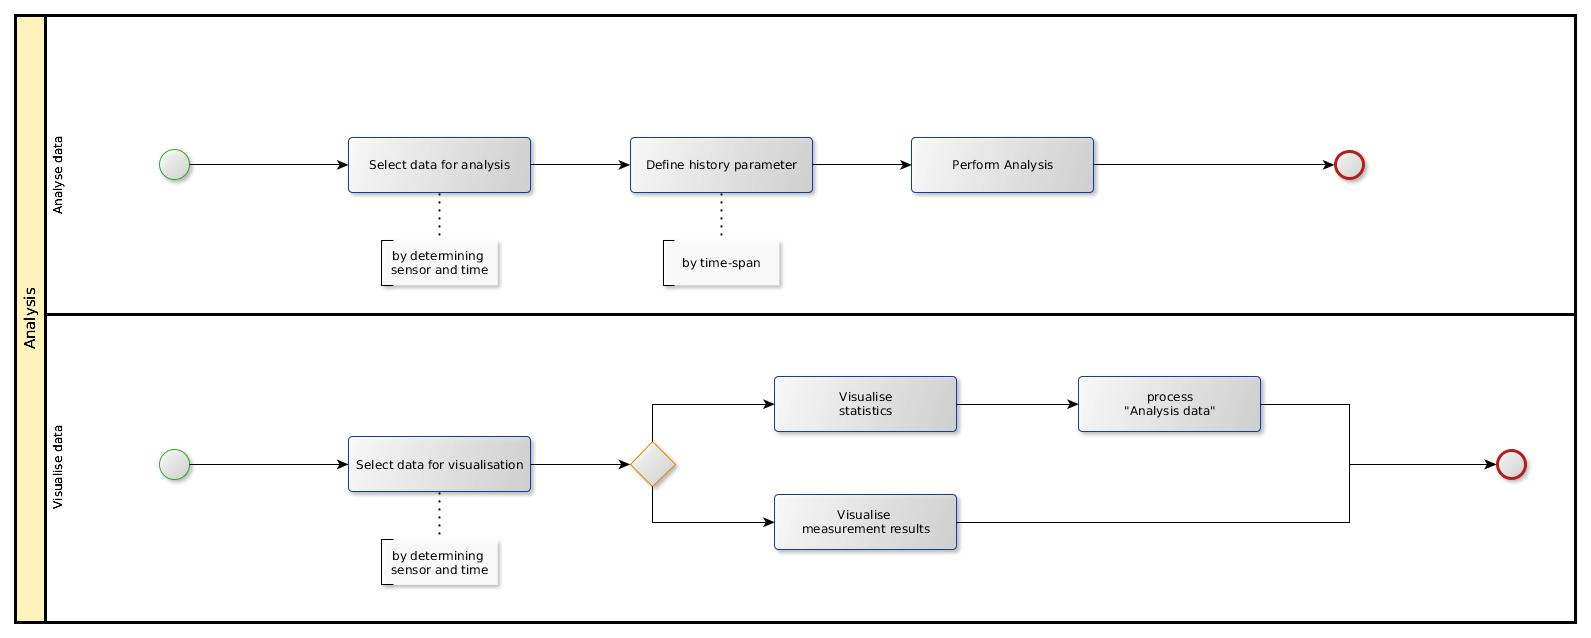
\includegraphics[scale=0.24]{graphics/bpmn_use-cases_analysis.jpg} 
	\caption{BPMN (Business Process Model and Notation) Model of the use cases describing central analysis proceedings. By F. H. Euteneuer 2013}
	 \label{fig:bpmn_use-case_analysis}
\end{figure}


\section{Product functionalities}
This part will describe the non-functional requirements of the system. This can be understood as a description of where the system will operate and how the software will operate. Non-functional requirements are requirements on a system which are not a technical functionality but a feature of the system.

The following list is describing those non-functional requirements:

\begin{description}
\item[portability] Since the system will be based on mobile devices, and those are not in any case running under windows, the software will be platform independent. Nevertheless also a web-based system is not possible, because the necessary internet connection will not be permanently available in field.
\item[performance] As described in the point before, the system will use different mobile platforms. Those do not have a hardware with a hight performance. Therefore the systems mobile part will be planed for a low performance.
\item[simplicity] The system will be used from field engineers which are working often under lots of negative influences of the environment. The system will be constructed as simply as possible to avoid unnecessary time costs for searching the right systems functionality.

\end{description}


\subsection{Fundamentals of Photovoltaik systems}

A Photovoltaic systems transduces solar radiation into electricity. The efficiency of a system depends on the properties of the used photovoltaic cells. Wagner (2010) \citen{Wagner2010} \\

\begin{figure}[hbt!]
\centering
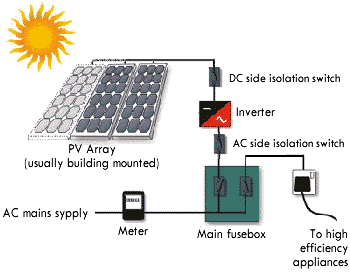
\includegraphics[width=0.7\textwidth]{phase2/group2/figure/pv-system-configuration.png}
\caption{Architecture of Photovaltaic system}
\label{fig:PV_system}
\end{figure}

The nominal power of a cell is given in Watt and often denoted as \(W_p\) (Watt Peak). It is acquired under standard test condition (STC an international standard) from the manufacturer of the photovoltaic cell. STC means, that the cell temperatur is \(25^\circ C\) and the irradiance is 1000 \(W/m^2\). The nominal power can be used to compare the power of photovoltiac cells of different manufactures. 
\\
The efficiency is given by the ratio between the produced energy and the energy radiated to the cell. It depends on the temperature of the photovoltaic cells. With increasing temperature the efficiency decreases. Often only one efficiency coefficient, including the efficiency of the power inverter, cable and accumulator, is given by the manufacturers.
\\
In addition a performance ratio is given most times. It is the ratio of the actual and the desired gain of the photovoltaic cell. It depends not only on the cell itself but also on the weather conditions, respectivly on the location. The desired gain is the efficiency of the installation under STC, assuming that the efficiency of the power inverter is \(100\%\). For a thin-layerd slicon cell, which is most common, the Performance ratio (PR) is \(84\% \) for Germany.
Wagner (2010)


\subsection{Fundamentals of Solar thermal systems}

Solar thermal collectors are devices, which transform radiation emitted by sun into heat. Basically, a collector consists of a box with a black glazed cover, containing a pipe, which uses all the space in the box. The radiation is adsorbed by the black glazing and heats up a fluid, such as water or oil, which runs through the pipe equipped in the  collector. The heated fluid can then be stored in insulated tanks, if it cannot be used directly.    In general solar collectors are used for use water in a household or for heating.\citen{Kalogirou}

basically, the efficiency of a solar thermal collector depends on the absorption of the glazing, the input fluid temperature , the average air temperature as well as the solar radiation of the region.
% global irradiance
\subsection{Global Irradiance}

The most important input value to calculate the Solar potential is the global radiation. The global radiation comprises the direct solar radiation and the diffuse radiation resulting from reflected or scattered sunlight. It depends on the location, the orientation of the roof surface and the inclination of the roof surface. The location is the latitude \(52^\circ 31' 45.0''\) and longitude \(13^\circ 19' 42.6''\)  of Moabit in Berlin. The orientation and the inclination are calculated from the CityGML Lod2 geometry. (European Database of Daylight and Solar Radiation)

\subsubsection{Orientation of the roof}

The azimuth angle \(\alpha\) represents the orientation of the roof. It is given by the angle between the normal vector of the roof \(n_r\) surface and the normal vector of xz plane \(n_{xz}\). 
\begin{eqnarray}
\label{eq:angle2vec}
\alpha = cos^{-1} ( \frac{\vec{n_r} \vec{n_{xz}}}{|n_r|  |n_{xz} | })
\end{eqnarray}

The direction of the normal vector is defined by the order of the point sequence forming the polygon ring of the roof surface. To calculate the orientation the positive normal vector is needed. If \(n_r\) has a negative z component \(n_r\) is converted to the positive normal vector. The calculated angle \(\alpha\) is always in a range between \(0^\circ-180^\circ\). Because the azimuth angle has a range of \(0^\circ-360^\circ\) we have to consider the sign of the x component of \(n_r\). Is the x component negative the azimuth angle is calculate with
\begin{eqnarray}
\alpha_o = 360^\circ - \alpha
\end{eqnarray}
else the azimuth angle \(\alpha_o\) is equal to \(\alpha\). 

\subsubsection{Inclination of the roof}
The inclination of the roof influences the input of solar radiation strongly and has to be considered. It is calculated as the angle between the normal vector of the roof surface \(n_r\) and the normal vector of the xy plane \(n_{xy}\). To calculate this angle equation \ref{eq:angle2vec} is used. Again the calculated angle ranges between \(0^\circ-180^\circ\), although the maximal tilt angle is \(90^\circ\). Therefore the tilt angle is
\begin{eqnarray}
t = 180^\circ - \alpha 
\end{eqnarray}
if \(\alpha > 90^\circ\) else \(t\) is equal \(\alpha\). For further calculation all roof surfaces with an inclination \(t<8^\circ\) are considered to be flat roofs and the angle \(t\) is set to \(0^\circ\).

\subsubsection{Satel-Light Database}
The estimation of the global irradiation for flat roof surfaces is simple, because no diffuse radiation effects the global radiation. For inclined surfaces the diffuse radiation resulting from reflected or scattered sunlight has to be considered. Because this is very complex we decided to use the European Database of Daylight and Solar Radiation (Satel-Light), which provides for every location within Europe the global radiation on tilted else well as flat roof surfaces with arbitrary orientation. We created a LookUp table for Berlin, which contains the global radiation for the inclination in \(10^\circ\) degree steps and the orientation in \(45^\circ\) steps. The resulting table is shown in figure \ref{fig:rad_table}.

\begin{figure}[hbt!]
\centering
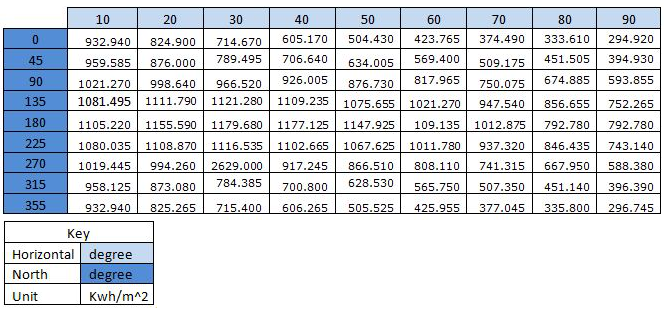
\includegraphics[width=0.9\textwidth]{phase2/group2/figure/table_global_radiation.png}
\caption{LookUp table for the global radiation for Berlin}
\label{fig:rad_table}
\end{figure}

\subsection{Reduction of Roof Surface Area due to Roof Equipment}
\label{sec:roofarea}
The main problem when using a LOD 2 model is that the suitable roof area is not known. Fact is, that not 100\% of the roof can be used to install solar panels, since roofs may have dormers, antennas or chimneys which are not part of the LOD2 model. But the roof equipment is considered for the Solar Atlas Berlin and with use of this data source empirical reduction factors may be computed. Therefore group 2 implemented a program, which reads a cityGML file, containing all buildings of the test area (~1000 buildings) and computes the reduction factor as in Equation \ref{eq:roof}.

\begin{align}
\label{eq:roof}
r_E &= \frac{A_{SAB}}{A_{LOD2}} \\\notag\\\notag
\text{with:}&\\\notag
r_E &:\text{ empirical reduction factor}\\\notag
A_{SAB} &: \text{Roof Area according to solar atlas Berlin }\\\notag
A_{LOD2} &: \text{ roof area calculated from LOD2 model in 3D CityDB }\\\notag
\end{align}

The Solar Atlas Berlin provides different areas for photovoltaic and solar thermal systems. Therefore also different reduction factors are computed. The reduction factors are also separated between exclusively flat roof and mixed roofs, contain flat as well as tilted surfaces. This is important because flat roofs are more likely equipped. Additionally, the age class of the building has been taken into account. Tables \ref{tab:roofarea_st} and \ref{tab:roofarea_pv} show the result, including the number of surface and the variance of the value. It can be seen that, some reduction factors are not representative, because not enough roofs of this type are in the test area. With the use of a database of entire Berlin might fix the Problem.

 

\begin{table}
\centering 

\begin{tabular}{|c||c|c|c||c|c|c|}
  \hline
  \multirow{2}{*}{Age Class} & \multicolumn{3}{|c||}{flat roof} &  \multicolumn{3}{|c|}{mixed roof}\\
  \cline{2-7}
  & $r_E$ & count & $\sigma^2$  & $r_E$ & count & $\sigma^2$\\
  \hline
1899&0.198&94&0.016&0.440&199&0.056\\\hline
1918&0.152&56&0.019&0.435&233&0.059\\\hline
1932&0.167&13&0.017&0.506&9&0.048\\\hline
1945&0.304&2&0.0008&0.765&1&0.000\\\hline
1961&0.221&74&0.013&0.581&56&0.049\\\hline
1974&0.198&90&0.015&0.371&17&0.080\\\hline
1993&0.219&66&0.006&0.293&5&0.016\\\hline
2012&0.149&91&0.019&0.487&21&0.165\\\hline
\end{tabular}
\caption{empirical reduction factors for calculation of energy gain using solar thermal collectors }
 \label{tab:roofarea_st}
\end{table}

\begin{table}
\centering 
\begin{tabular}{|c||c|c|c||c|c|c|}
  \hline
  \multirow{2}{*}{Age Class} & \multicolumn{3}{|c||}{flat roof} &  \multicolumn{3}{|c|}{mixed roof}\\
  \cline{2-7}
  & $r_E$ & count & $\sigma^2$  & $r_E$ & count & $\sigma^2$\\
  \hline
1899&0.127&94&0.019&0.349&199&0.050\\\hline
1918&0.097&56&0.016&0.323&233&0.053\\\hline
1932&0.056&13&0.008&0.403&9&0.076\\\hline
1945&0.000&2&0.000&0.730&1&0.000\\\hline
1961&0.147&74&0.015&0.498&56&0.050\\\hline
1974&0.129&90&0.016&0.289&17&0.081\\\hline
1993&0.128&66&0.011&0.146&5&0.013\\\hline
2012&0.090&91&0.016&0.399&21&0.147\\\hline
\end{tabular}
\caption{empirical reduction factors for calculation of energy gain using photovoltaic modules }
 \label{tab:roofarea_pv}
\end{table}


\subsection{Shadowing}
\label{sec:shadowing}
Roof surfaces may be shadowed by several object, such as other buildings, trees or even equipment on the roof itself. Since, the data source is a LOD 2 model only other buildings can be considered, because trees and roof equipment are not part of the model. The consideration of the shadowing may be done with a complicated illumination computation. Since this project is limited in time this is not possible. Therefore only a simple approach is applied, which completely ignore buildings which are shadowed, rather then adjusting the daily global irradiance on the specific surface.
Within the simple approach a building is neglected, if there is a neighboured building which is $x$ higher and is within a certain radius $r$. Only buildings between an azimuth of 90° to 270° are taken into account, as shown in Figure \ref{fig:shadow}.

\begin{figure}[ht]
	\centering
	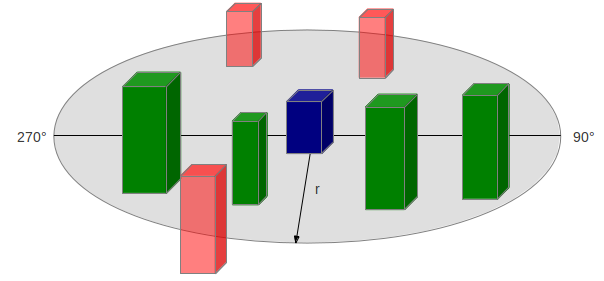
\includegraphics[width=0.7\textwidth]{phase2/group2/figure/fig_shadow.png}
	\caption{The green buildings are candidates, which may shadow the blue building}
	\label{fig:shadow}
\end{figure}

The implemented algorithm starts with iterating over all buildings and storing them in a spatial tree to make them easy queryable. After that before a potential of a building is calculated it will be checked if there are candidate buildings which are within the radius $r$. The list of candidates is checked for buildings which also meet the other conditions, such as an azimuth between $90^\circ$ and $270^\circ$ and if the building is $x$ times higher. If both conditions are met, the building will be neglected for the potential calculation. 
\subsection{Calculation of the potential}

The calculation begins with the reduction of the roof area according to the building age class as described in chapter \ref{sec:roofarea}. If the roof surface is a flat roof ($tilt < 8 ^\circ$) the modules cannot directly mounted of the roof surface. To bring the modules in an optimal tilt angle they are mounted on a mounting system of the roof. Because they are tilted they might shadow the neighboring modules, therefore a certain distance between the modules is necessary as shown in Figure \ref{fig:flatroof}. The distance has to be $c=2.75$ times longer then the width of the ground of the module $w$.
%TODO: ADD REFERENCE!
\begin{figure}[ht]
	\centering
	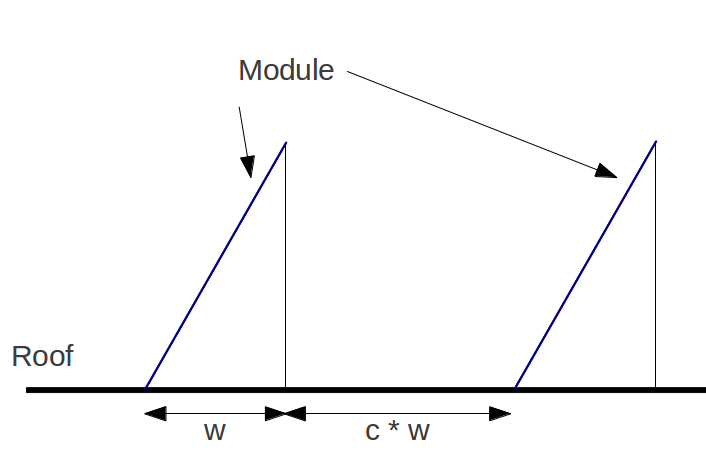
\includegraphics[width=0.5\textwidth]{phase2/group2/figure/flatroofreduction.png}
	\caption{Solar Modules mounted on a mounting system of a flat roof}
	\label{fig:flatroof}
\end{figure}
Furthermore the global irradiance has to be picked from the look-up table. According to Solar Atlas Berlin \citen{solaratlas} areas with a global irradiance less than $905 Wh/m^2$ have to be neglected. Also surface are neglected which have a smaller area then $5m^2$. It is assumed that it is economically not worth the mount modules on such a small roof. The actual calculation of the potential highly depends on the type of module. This will be explained in the following sub sections.



\subsubsection{Potential of Photovoltiac systems}
To calculate the potential of photovoltiac systems two approaches were applied. First the estimation as described by Wagner (2010) \citen{Wagner2010} was implemented. According to Wagner (2010) the energy gain of a photovoltiac system can be calculated with 

\begin{align}
\label{eq:pv_calc}
E &= M \cdot GA \cdot \frac{P}{E_0} \cdot PR \cdot \eta_{EUR} \cdot \eta_l \\\notag\\\notag
\text{with:}&\\\notag
E &:\text{total energy gain per year \(kWh/a\)} \\\notag
E_0 &:\text{1000 \(W/m^2\)} \\\notag
M &:\text{Number of Modules} \\\notag
PR &:\text {Performance ratio} \\\notag
P &:\text{nominal power \(W\)} \\\notag
\eta_{EUR} &:\text{euro inverter efficiency} \\\notag
\eta_l&:\text{transmission efficiency} \\\notag
GA &:\text{Global Irradiation \(kWh/m^2 a\)} \notag
\end{align}

The parameters \(P\),\(\eta_{EUR}\),\(\eta_l\) and \(M\)depend on the photovoltaic cell and the inverter. Values for these parameters are taken from real photovoltiac cells. For the calculations the silicon cell BP 585F from BP Solar \citen{BPSolar} combined with the inverter SP 2500-450 from the company Sun Power \citen{SunPower} has been used. The inverter efficiency is \(\eta_{EUR} = 15 \%\) and the transmission efficiency is set to \(\eta_l = 9\%\). The nominal power of the cell is \(P_0 = 85 W\). This calculation method allows to use real data of photovoltiac cells and considers the inverter.
\\

Because the the Solar Atlas Berlin is the only available reference, finally a second approach according to the Solar Atlas was used. The calculation of the photovoltiac energy is simplified and finally done with equation \ref{eq:pv_calc_SAB}. Where the efficiency coefficient is set to \(e=15\%\) and the system area is the reduced roof surface area.

\begin{align}
\label{eq:pv_calc_SAB}
E &= A \cdot GA \cdot PR \cdot e \\\notag\\\notag
\text{with:}&\\\notag
E &:\text{total energy gain per year \(kWh/a\)} \\\notag
A &:\text{System Area \(m^2\)} \\\notag
e &:\text{efficiency coefficient} \\\notag
GA &:\text{Global Irradiation \(kWh/m^2 a\)} \notag
\end{align}





\subsubsection{Solar Thermal}
The calculation of the potential of solar thermal modules was done as described in Struckmann (2008) \citen{struckmann2008}. According to Struckmann (2008) the useful energy gain $Q_U$ of a solar thermal module is calculated with the formula shown in Equation \ref{eq:st_calc}. Figure \ref{fig:st_module} shows a sketch of a typical solar thermal module and shows the parameter, which are necessary to compute $Q_U$  

\begin{align}
\label{eq:st_calc}
Q_U &= F_R  A \left( I \tau \alpha - U_L \left(T_i - T_a \right) \right)\\\notag\\\notag
\text{with:}&\\\notag
F_R &:\text{ Efficiency Coefficient of the module}\\\notag
A &: \text{ module area, $m^2$}\\\notag
I &: \text{ Solar radiation, $W/m^2$ }\\\notag
\tau &: \text{ transmission coefficient of glazing}\\\notag
\alpha &: \text{ absorption coefficient of plate}\\\notag
U_L &: \text{ collector overall heat loss coefficient, $W/m^2$}\\\notag
T_i &: \text{ input fluid temperature, $^\circ C$}\\\notag
T_a &: \text{ average outside air temperature, $^\circ C$}\notag
\end{align}

\begin{figure}[ht]
	\centering
	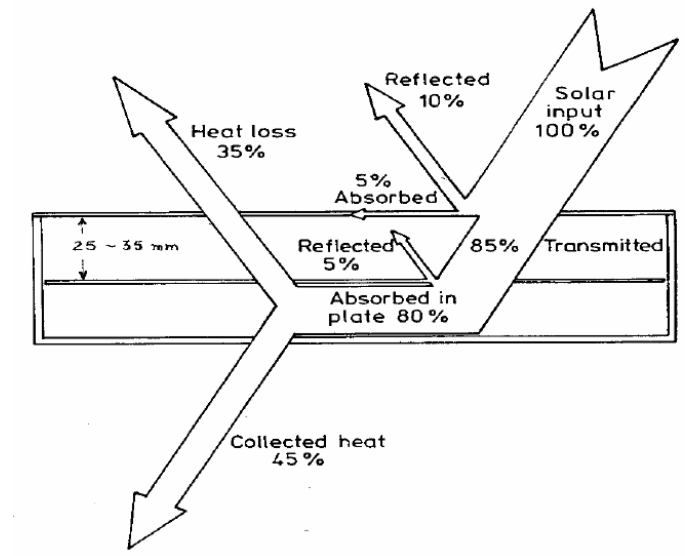
\includegraphics[width=0.5\textwidth]{phase2/group2/figure/st_module.png}
	\caption{typical module with visualization of calculation parameters (Struckmann (2008))}
	\label{fig:st_module}
\end{figure}

For the calculation of the potential a standard solar thermal module has been taken, the TitanPower-AL2DH Flat Plate Collector from the company SunMaxxSolar \citen{sunmaxx}. The efficiency coefficient is assumed to be $F_R = 0.35$ since this value is also used by SimuPLAN for Solar Atlas Berlin. The input fluid temperature is assumed to be $T_i = 10 ^\circ C$ which seems to be a realistic value for the region of Berlin.  Also the average outside air temperature is taken as  $T_a = 10 ^\circ C$.



\subsection{Validation of Result}
The results are compared and validated against the values computed for the project "Solar Atlas Berlin". According to the roof area which is suitable for solar panels per building, the geometry data source of the Solar Atlas is expected to be of higher quality, because the data has been acquired using a laser scanning system. Therefore, the usable roof area may be exactly predicted for each building. Usable roof area is the area which is not used for any equipment on the roof, such as dormer, chimneys or antennas. The data source used within the GIS Project is an LOD2 Model of Berlin, which does not contain information about roof equipment. For this reason, we use the Solar Atlas Berlin to validate our results.

The value which is validated is calculated potential in MWh/a for photovoltaic systems as well as solar thermal systems. For each building in the test area the difference between the potential given from Solar Atlas Berlin and the potential calculate within the project in calculated. Note, that photovoltaic and solar thermal system are always considered separately.

Out of the differences, the standard deviation can be computed. Since the expectation is known ($e=0$, no difference) the standard deviation is computed as in Equation \ref{eq:validation}.

\begin{align}
\label{eq:validation}
\sigma = \sqrt{\frac{1}{n} \sum\limits_{i=1}^n (diff_i - e )^2}
\end{align}

For the test area a standard deviation of $\sigma_{pv} = 6.45 Mwh/a$ for photovoltaic and $\sigma_{st} = 10.49 Mwh/a$ for solar thermal systems has been reached. A weak spot of this approach is, that outliers influence the result. Although most of the differences are close to zero, the standard deviation is relatively high.
\subsection{Visualization}

To visualize the results a new appearance theme is added using citygml4j. To do this the results have to be classified. For both photovoltaic and solar thermal potential three classes are defined.
\\
Photovoltaic
\begin{itemize}
\item Photovoltaic potential classes
\subitem \(>=50kWh/m^2a\), very good, color: red
\subitem \(<50kWh/m^2a\), good, color: orange
\subitem \(<30kWh/m^2a\), limited, color: yellow
\item Solar thermal potential classes
\subitem \(>=100kWh/m^2a\), very good, color: red
\subitem \(<100kWh/m^2a\), good, color: orange
\subitem \(<50kWh/m^2a\), limited, color: yellow
\end{itemize}

Due to time problems the classification is not optimal. The class boundaries are only empirical values. Furthermore the total energy output depends on the roof area. Which leads to a classification of small roofs to low class although the orientation optimal and the global radiation high. For further investigations this classification should be optimized. The Solar Atlas Berlin uses total global radiation to classify the potential, which could be used as better model.
The new appearance theme is created with citygml4j. Each roof surfaces is added as appearance member. According to the class the are linked with the corresponding diffuse color.
After writing the new CityGML file with all energy related attributes and the new appearance theme. The file is imported to a empty database. Subsequently a KML/Collada export is used to export a KML file with the new appearance IGG\_PV\_Potential. Additionally the address and the values of photovoltaic and solar thermal potential are stored in KML balloons for each building. Figure \ref{fig:vis} shows the resulting KML of the statistical block in Google Earth.

\begin{figure}[hbt!]
\centering
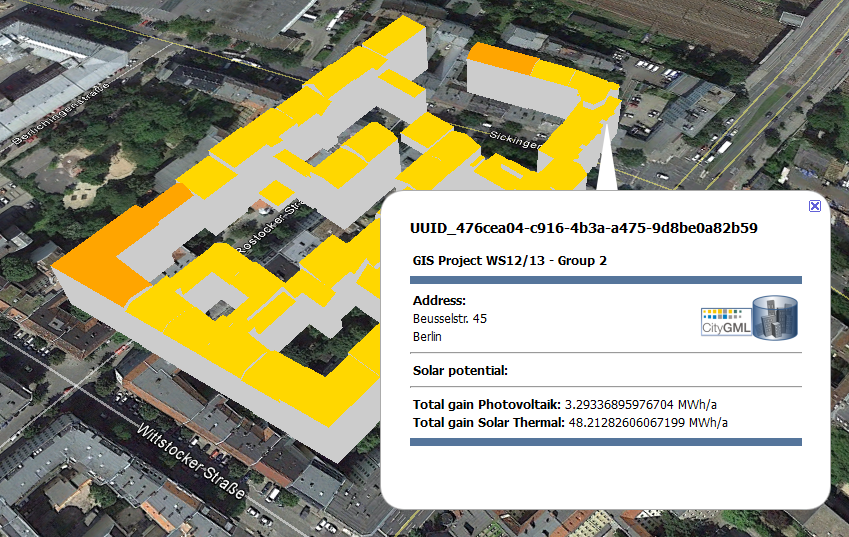
\includegraphics[width=0.7\textwidth]{phase2/group2/figure/viz.png}
\caption{KML export}
\label{fig:vis}
\end{figure}

\subsection{Conclusion}
% TODO: point out weak spots of our implementation and validation (e.g. Solar Atlas is not reliable enough, roof surfaces are not merged)
It can be concluded that the estimation of the photovoltaic potential as well as the solar thermal potential is only applicable to a limited extend. For single buildings the estimation is far to inaccurate, whereas the results for a statistical block become more reliable. The standard deviation for both potentials is too high, it is close to the mean of the potential, which means the result is for a high percentage of all buildings is totally wrong. But the standard deviation is calculated on the basis of the values given by the Solar Atlas Berlin. Therefore the values of the Solar Atlas Berlin are assumed to be correct. That this is not always the case was proved at least with on building. The potential was shifted by one decimal place. Also the geometry data is not sufficient. The used Lod2 (Level of detail 2) geometry only comprises simple polygons to describe the roof surfaces. No geometry of additional roof structures, as dormers, antennas or chimneys are  available. Furthermore the roof surfaces 
representing one roof within the 3D City DB does not always correspond to the real roof surfaces. Some roof surfaces are represented by several small surfaces in the Database. This leads to errors for the estimation of the potentials, because horizontal roof surfaces smaller \(40m^2\) and tilted roof surfaces smaller \(15m^2\) are ignored during the calculation of the potential. \\
The solar potential of roofs depends strongly on the input of solar radiation, which in turn is strongly influenced by shadows. The used shadowing model is very simple. Only shadows due to very high neighboring buildings are considered. Shadows due to additional roof construction are neglected. Tests showed that only a few buildings were neglected due to the implemented shadow model. \\
Nevertheless the estimation of solar potential with existing CityGML data can be very fast and cheap, because no expansive Lidar data is necessary.\\
For the current implementation the disadvantages outbalance the advantages. The results are not accurate enough to use this approach 
\subsection{Future Work}
%TODO: things which may be implemented to improve the results. describe possible solutions to fix the  ``weak spots'' which we pointed %out in the conclusion.

Further investigations to improve the calculation model can lead to better results. Instead of an Lod 2 geometry a higher level of detail as Lod 3 can be used, which describes the geometry of the roofs in more detail. To avoid the neglection of too small roof surfaces due to wrong surface separations, neighboring roof surfaces with equal inclination and orientation should be merged in future.\\
In addition a high order shadow model, which considers partly shadowing of a roof surfaces due to other buildings and shadowing due to additional roof structures. Until now the shadow model is not capable of reducing the global irradiation, but neglects the whole building. The new model should be able to deal with this reduction due to partly shadowed roof surfaces.

%\end{document}

\newpage

\chapter{
\section{Estimation of Residential Electricity Consumption Based on 3D City Model}
}%group 3
\subsection{Define Algorithm}

Normally, the algorithms used to calculate the electricity consumption depend on a large amount of variables and factors, as can be seen on figure 7: \citep{costa2012} \\

\begin{figure}[htb!]
	\centering
	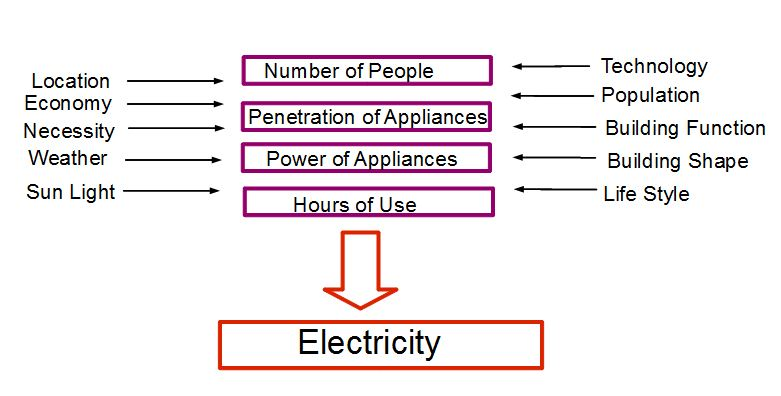
\includegraphics[width=0.8\textwidth]{phase2/group3/fig8.png}
	\caption{Factors for calculating the electricity consumption (Costa, 2012) }
	\label{fig:figure8}
\end{figure}

According to this sketch, in order to calculate the electricity consumption, except the number of people, it is required to know the penetration of appliances, the power of appliances and the hours of use. Such data are changed from one situation to another. The available data cannot support this algorithm, and, therefore, some assumptions are done in order to simplify the process.

According to this situation, a new algorithm is created to estimate the annual consumption based on different household. Figure 9 illustrates the annual consumption for different number of household. Since the number of apartment and residents in each building already calculated in Phase I. If  the residents can be distributed into each apartment as household, the electricity consumption can be calculated from it.

\begin{figure}[H]
	\centering
	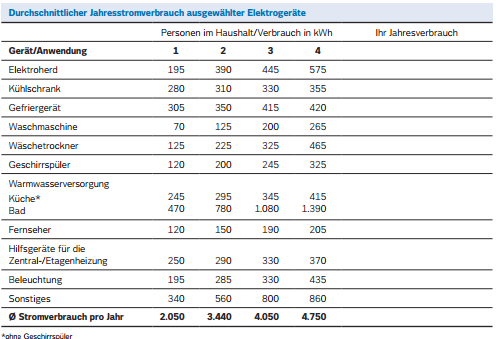
\includegraphics[width=0.8\textwidth]{phase2/group3/fig9.png}
	\caption{The annual electricity consumption for different number of household (Vattenfall 2012) }
	\label{fig:figure9}
\end{figure}

\subsection{Data Source}
From Phase I, the results are mainly two indicators: Apartments/volume and Resident/ Building. If these two indicators are applied to all the residential buildings, the number of apartments per buildings will be get. Also the average share of household in Mitte can be found in statistic department.\citep{statsberlin} Combining the electricity consumption data from Vattenfall, all the data for estimating the annual consumption is provided.

\subsection{Method}
Figure 8 illustrates the work flow for calculate the results as well the data sources:

\begin{figure}[htb!]
	\centering
	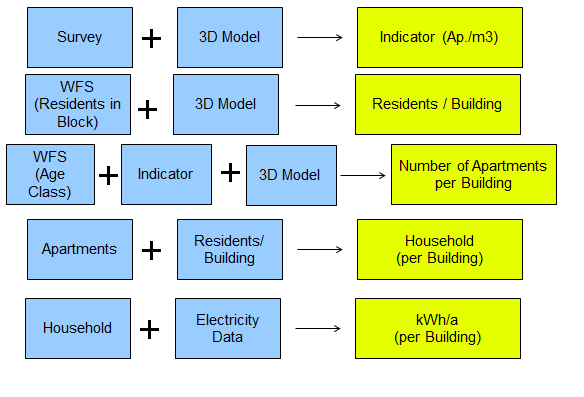
\includegraphics[width=0.6\textwidth]{phase2/group3/fig10.png}
	\caption{Workflow for Phase II }
	\label{fig:figure10}
\end{figure}

For the last step, there are two ways to calculate the electricity:
1) Establish the regression equation and apply the average household in the equation (see figure 10). This equation was created from the data available on Figure 8.

\begin{figure}[H]
	\centering
	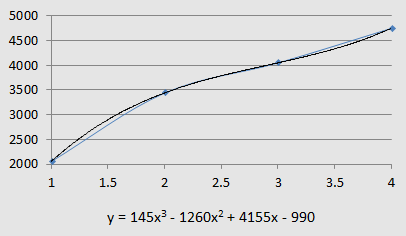
\includegraphics[width=0.6\textwidth]{phase2/group3/fig11.png}
	\caption{The regression equation for electricity consumption}
	\label{fig:figure11}
\end{figure}

2) Distribute the residents into each apartment to get the number of apartment with different household. And use these numbers to multiply the corresponding electricity and lighting consumption. This distribution is base on the statistical share of households for the giving area.

\subsection{Household Distribution}
One of the most important parts in the second method is distributing the inhabitants into apartment. There are three inputs already known: the apartment number, the residents number and the average share of different household. To distribute the residents, only two variables above can be fixed with one variable left. Therefore there are three methods: 

\begin{itemize}
\item Fix the share and residents number, take apartment number as variable
\item Fix the share and apartment number, take residents number as variable
\item Fix the apartment and residents number, take share as variable
\end{itemize}

While for the first two methods the variable parameters will be changed in a unreasonable way, and make the results not reliable, a new distribution method is developed from the third method. 

\subsubsection{Basic Idea}
The basic idea of this method is to try to keep the share close to the average share of Mitte, by applying the following steps:\\
\\
1. Spit the total number of apartment with different household based on the percentage \\
2. Check how many residents left\\
3. Distribute the left residents\\
4. Keep the ratio of the 2~4 household: 3:1:1

\subsubsection{First Distribution}
After the first distribute based on the share, there will be three difference scenes:\\
\begin{itemize}
\item $R > 0$   more people live in one apartment
\item $R < 0$   less people live in one apartment
\item $R < Apartment$  only household(1) and empty apartment
\end{itemize}

In the last scenes, all residents will be put into each apartment with only 1 household and the other apartments are empty. For the first and second scenes, the left residents have to be distributed again.

\subsubsection{Second Distribution}
In the second distribution, as can be seen in figure 11, if only one residents left, it will be put into an apartment with 1 household, which means the number of 1 household will decrease 1 and the number of 2 household will increase 1. If two left, put both of them into 1 household. And the number of 1 household will also decrease 1 but the number of 3 household will increase 1. Do the same as shown in the figure 11 until 8. if there are 9 left, distribute the first 8 as -5:3:1:1 then put the left 1 to 1 household. \\
By this distribution method, it keeps the ratio of the 2~4 household as 3:1:1, which also means every 8 residents as a loop. 


\begin{figure}[H]
	\centering
	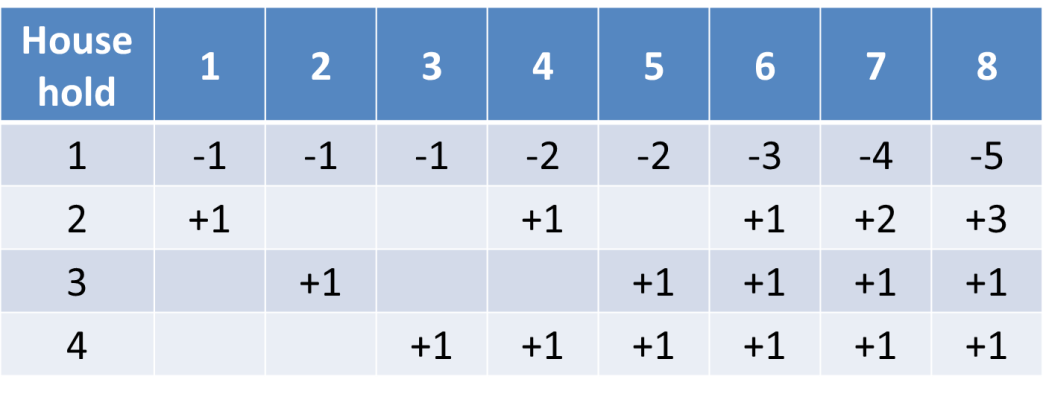
\includegraphics[width=0.8\textwidth]{phase2/group3/fig12.png}
	\caption{The second residents’ distribution method (Self Made)}
	\label{fig:figure12}
\end{figure}

\subsection{ArcPython User Interface}

To apply this method to other dataset, an Arctool was designed by using python script which has a good connection with ArcGIS 10. 

\begin{figure}[ht]
	\centering
	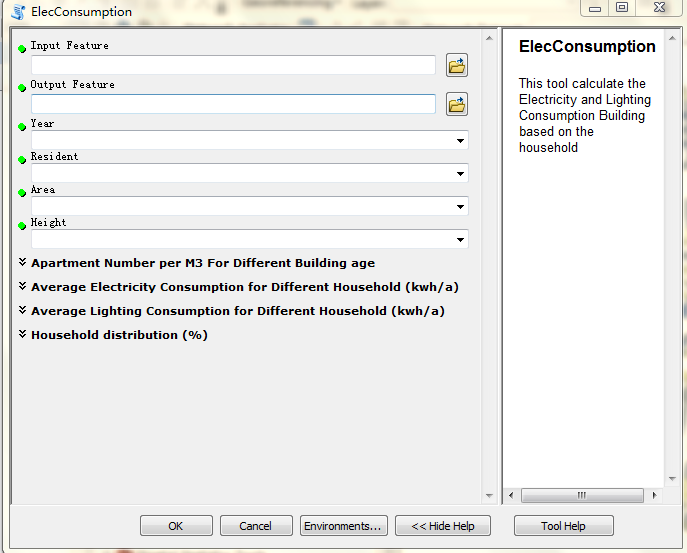
\includegraphics[width=0.8\textwidth]{phase2/group3/fig13.png}
	\caption{Developed Arctool (Self Made)}
	\label{fig:figure13}
\end{figure}


\begin{figure}[H]
	\centering
	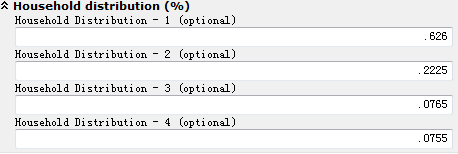
\includegraphics[width=0.8\textwidth]{phase2/group3/fig14.png}
	\caption{Developed Arctool - State Variables (Self Made)}
	\label{fig:figure14}
\end{figure}

The user can choose the input and output feature class and select the corresponding fields for building age, residents, area and height to calculate the electricity consumption. Besides, the user can also change the optional parameters such as the share of household and the annual electricity consumption for different household.

\subsection{Results}
After the resident distribution, the light and electricity consumption can be computed by multiplying the number of apartment with different household with corresponding consumption

\begin{figure}[ht]
	\centering
	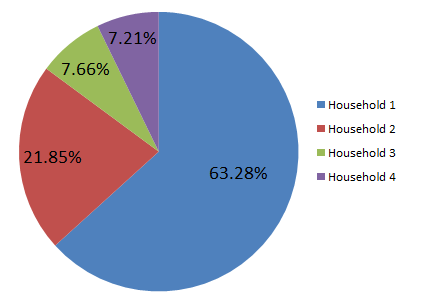
\includegraphics[width=0.7\textwidth]{phase2/group3/fig15.png}
	\caption{Final Household Share (Self Made)}
	\label{fig:figure15}
\end{figure}

\begin{figure}[ht]
	\centering
	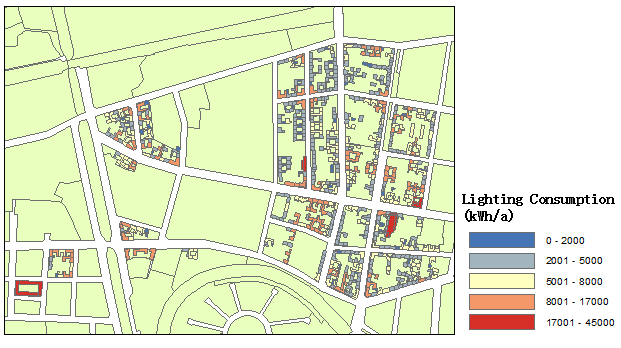
\includegraphics[width=1\textwidth]{phase2/group3/fig16.png}
	\caption{Final Lighting Consumption (Self Made)}
	\label{fig:figure16}
\end{figure}

\begin{figure}[H]
	\centering
	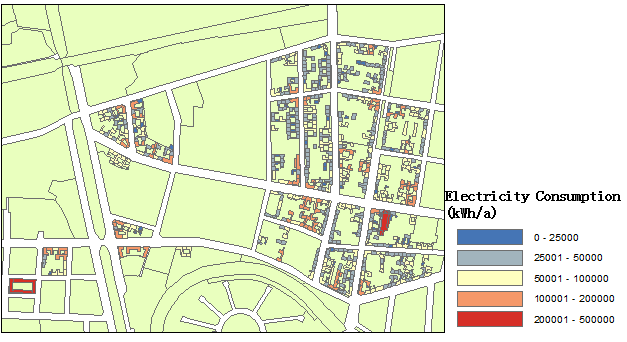
\includegraphics[width=1\textwidth]{phase2/group3/fig17.png}
	\caption{Final Electricity Consumption (Self Made)}
	\label{fig:figure17}
\end{figure}
\begin{figure}[H]
	\centering
	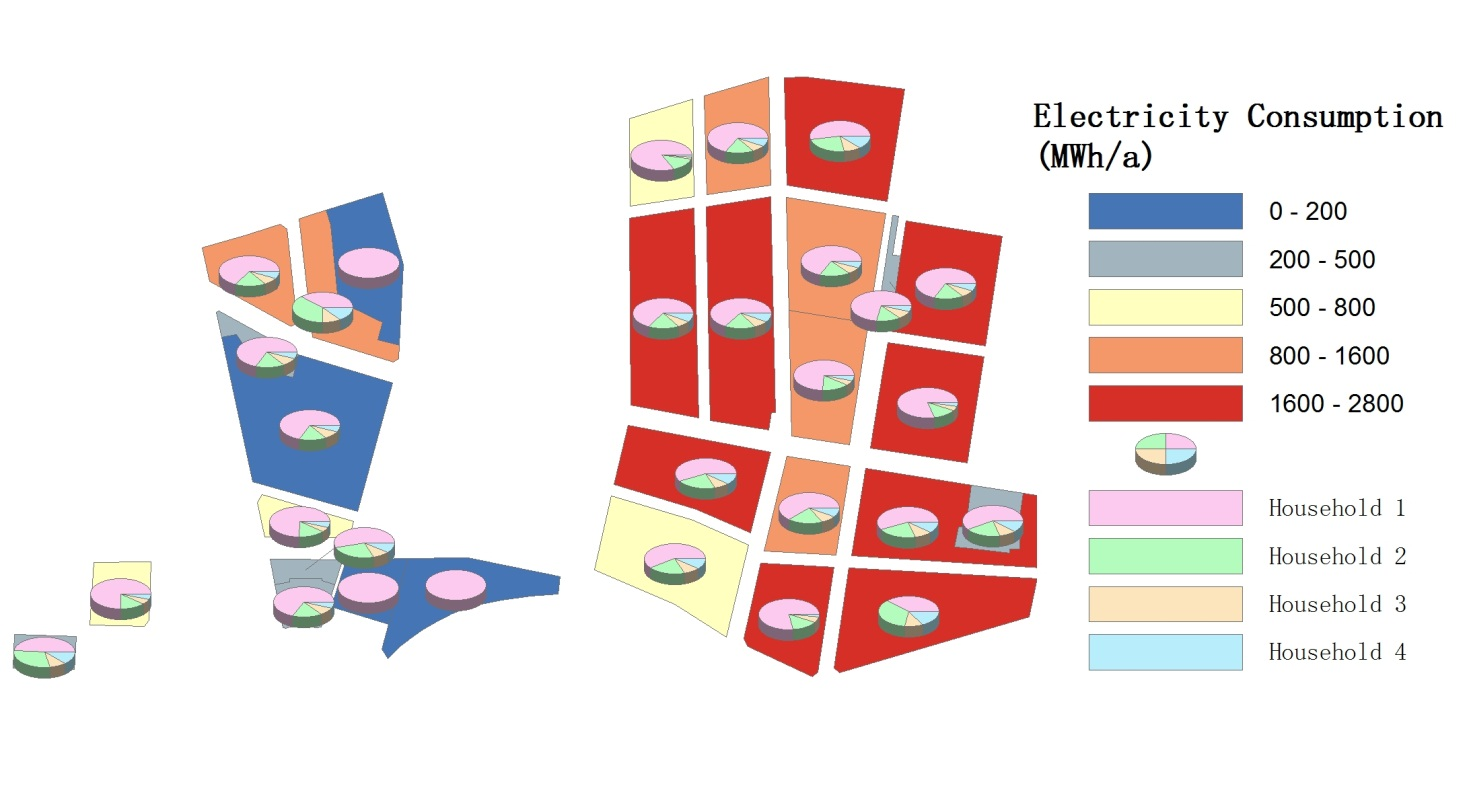
\includegraphics[width=0.9\textwidth]{phase2/group3/fig19.png}
	\caption{Final Electricity Consumption per Block (Self Made)}
	\label{fig:figure19}
\end{figure}
Table 2 shows the results from the two calculation methods. As can be seen from it, using the average household and regression equation the results are smaller than the distribution method. Nevertheless, both estimation methods rendered values within a short interval - as both are based essentially on the residents per building and/or per apartment. 


\begin{table}[H]
	\centering
	\includegraphics[width=0.8\textwidth]{phase2/group3/fig18.PNG}
	\caption{Final Electricity Consumption (Self Made)}
	\label{fig:figure18}
\end{table}



\subsection{Conclusion}
The described method is able to integrate statistical data, surveying data and virtual 3D City Models. Furthermore, it provides a rough tool to calculate the electricity for other area which can be implemented in 3D City Models. As a result, instead of having only average results, the calculations are also locally performed. In other words, as the parameters are first calculated per each building, it is also possible to select the final results for each building. The two distribution methods provide the user two different level results with different data. If there is no household share data, the regression equation method can give the rough results. While with the household share data, the distribution method can be applied for more reasonable results.\\

The 3D Model is able to provide all the demanded geometrical factors. Once the electricity consumption estimation is geometrically based on the volume of the buildings, data regarding its footprint area and height are required. \\

However, there still some parts need to pay attention to during applying this method. Such as the function of the building, the relationship between 3D City Model and the survey address.



\pagebreak
\bibliographystyle{plain}
\bibliography{references}{}
\end{document}
